\chapter{Operating System Layer}
\label{chap:os}
In the previous chapter we explore a design of memory management for disaggregated architecture in the service layer. However, integrating general application with an external memory service is challenging. In this chapter, we explore how to follow the class design of operating system, and leave the memory management functionality within the operating system. Transparency is an important aspect when considering migrating existing data center applications on disaggregated architecture.
The operating system layer plays a crucial role in supporting the core functionality of a disaggregated architecture. This includes tasks like thread scheduling and data movement (paging). One of the key questions that arises is where the operating system should be situated within this architecture. There are two main options to consider:

\paragraphb{Centralized OS Management} One approach is to place the operating system at a central point within the system, providing it with a global view. The advantage of this approach is that it maintains a well-defined operating system structure, requiring only minor modifications for application integration. However, ensuring that the central OS design doesn't introduce significant overhead is essential since the operating system typically lies on the critical path for applications, such as paging.

\paragraphb{Disaggregation of OS Functions} An alternative approach involves the disaggregation of operating system functions across various resource blades, a concept explored in ~\cite{legoos}. The rationale behind this approach is that many OS functionalities are closely intertwined with specific resources and remain largely independent of other system components. For instance, GPU driver functionality can be situated within GPU resource pools rather than near compute or memory nodes. While this approach offers enhanced flexibility, it requires a substantial effort to overhaul the operating system. It may introduce synchronization overhead due to the inherently distributed nature of the system, necessitating additional coordination.

In the upcoming subsections, we present a hierarchical OS design, combining elements from the previously discussed options. Subsequently, we delve into our validation efforts concerning centralized and disaggregated OS functionality. Finally, we introduce prospective avenues for future work.

\section{Hierarchical OS design}

Rather than exclusively opting for one of these two approaches, we advocate for a hybrid OS design that integrates elements from both options mentioned earlier. Our observation suggests that operating system functionality can be classified into two distinct groups:

\paragraphb{Non-disaggregated Functionalities} This category encompasses OS functionality that necessitates a holistic view of the entire system, including tasks like thread scheduling and memory management tasks such as memory address translation, protection, and paging. The operating system actively monitors the whole system, including available memory and compute resources, dynamically allocating computing and data resources to optimize system performance.

\paragraphb{Disaggregated Functionalities} In contrast, this category comprises OS functions closely intertwined with specific resource types, including memory, SSD, or GPU drivers. In these contexts, it is more logical to position the functionality near the respective resource itself. Regarding memory management, this entails the implementation of memory access optimizations, such as enhancing the speed of irregular memory access. These optimization processes do not interact with other system components, obviating the need for a global view of the system.

\section{In-Network Memory Management}
\subsection{Introduction}
The current state of data center network bandwidth is rapidly approaching parity with intraserver resource interconnects, with projections indicating an imminent surpassing of this threshold. This dynamic shift has ignited considerable interest within both academic and industrial circles towards memory disaggregation—a paradigm where compute and memory are physically decoupled into network-attached resource blades. This transformation promises to revolutionize resource utilization, hardware diversity, resource scalability, and fault tolerance compared to conventional data center architectures.

However, memory disaggregation presents formidable challenges, primarily revolving around three key requisites. Firstly, remote memory access demands low latency and high throughput, with previous studies targeting latency under 10 microseconds and bandwidth exceeding 100 Gbps per compute blade to minimize performance degradation in applications. Secondly, both memory and compute resources must exhibit elastic scalability, aligning with the essence of disaggregation. Lastly, seamless adoption and immediate deployment necessitate compatibility with unaltered applications.

Despite years of concerted research efforts directed towards enabling memory disaggregation, existing approaches have failed to concurrently meet all three requirements. Most strategies mandate application modifications due to alterations in hardware, programming models, or memory interfaces. Recent endeavors facilitating transparent access to disaggregated memory have encountered limitations on application compute elasticity—processes are confined to compute resources on a single blade to mitigate cache coherence traffic over the network, driven by performance apprehensions.

Introducing MIND, a pioneering memory management system tailored for rack-scale memory disaggregation, which effectively fulfills all three prerequisites for disaggregated memory. At the core of MIND lies a novel concept—embedding memory management logic and metadata within the network fabric. This innovative approach capitalizes on the insight that the network fabric in a disaggregated memory architecture essentially functions as a CPU-memory interconnect. In MIND, programmable network switches, strategically positioned for in-network processing, assume the mantle of Memory Management Units (MMUs), enabling a high-performance shared memory abstraction. Leveraging programmable hardware at line rate, MIND minimizes latency and bandwidth overheads.

However, the realization of in-network memory management necessitates navigating through the unique constraints imposed by programmable switch ASICs. These challenges include limited on-chip memory capacity, constraints on computational cycles per packet, and staged packet processing pipelines spread across physically decoupled match-action stages.

To address the trifecta of requirements for memory disaggregation, MIND ingeniously maneuvers through these constraints and harnesses the capabilities of contemporary programmable switches to enable in-network memory management for disaggregated architectures. This is achieved through a systematic overhaul of traditional memory management mechanisms:

MIND adopts a globally shared virtual address space, partitioned across memory blades to minimize the volume of address translation entries stored in the on-chip memory of switch ASICs. Simultaneously, it implements a physical memory allocation mechanism that evenly distributes allocations across memory blades for optimal memory throughput.

MIND incorporates domain-based memory protection, inspired by capability-based schemes, facilitating fine-grained and flexible protection by dissociating the storage of memory permissions from address translation entries. Interestingly, this decoupling reduces on-chip memory overheads in switch ASICs.

MIND adapts directory-based MSI coherence to the in-network setting, leveraging network-centric hardware primitives like multicast in switch ASICs to efficiently realize its coherence protocol.

To mitigate the performance impact of coarse-grained cache directory tracking due to limited on-chip memory in switch ASICs, MIND introduces a novel Bounded Splitting algorithm that dynamically sizes memory regions to constrain both switch storage requirements and performance overheads stemming from false invalidations.

The MIND design is realized on a disaggregated cluster emulated using traditional servers connected by a programmable switch. Results demonstrate that MIND facilitates transparent resource elasticity for real-world workloads while matching or even surpassing the performance of prior memory disaggregation proposals. However, it's noted that workloads characterized by high read-write contention exhibit sub-linear scaling with additional threads due to the limitations of current hardware. Present x86 architectures hinder the implementation of relaxed consistency models commonly employed in shared memory systems, and the switch TCAM capacity nears saturation with cache directory entries for such workloads. Potential approaches for enhancing scalability with future advancements in switch ASIC and compute blade architectures are discussed.
\subsection{Background and Motivation}
This section motivates MIND. We discuss key enabling technologies, followed by challenges in realizing memory disaggregation goals using existing designs.

Assumptions: We focus on memory disaggregation at the rack-scale, where memory and compute blades are connected by a single programmable switch. We restrict our scope to partial memory disaggregation: while most of the memory is network-attached, CPU blades possess a small amount (few GBs) of local DRAM as cache.

2.1 Enabling Technologies
We now briefly describe MIND’s enabling technologies.

Programmable switches: In recent years, programmable switches have evolved along two well-coordinated directions: development of a flexible programming language for network switches and the design of switch hardware that can be programmed with it. These switches host an application-specific integrated circuit (ASIC), along with a general-purpose CPU with DRAM. The switch ASIC comprises ingress pipelines, a traffic manager, and egress pipelines, which process packets in that order. Programmability is facilitated through a programmable parser and match-action units in the ingress/egress pipelines.

The program defines how the parser parses packet headers to extract a set of fields, and multiple stages of match-action units process them. The general-purpose CPU is connected to the switch ASIC via a PCIe interface and serves two functions: (i) performing packet processing that cannot be performed in the ASIC due to resource constraints, and, (ii) hosting controller functions that compute network-wide policies and push them to the switch ASIC.

While this discussion focuses on switch ASICs with Reconfigurable Match Action Tables (RMTs), it is possible to realize MIND using FPGAs, custom ASICs, or even general-purpose CPUs. Each exposes different tradeoffs, but we adopt RMT switches due to their performance, availability, power, and cost efficiency.

DSM Designs: Traditionally, shared memory has been explored in the context of NUMA and distributed shared memory (DSM) architectures. In such designs, the virtual address space is partitioned across the various nodes, i.e., each partition has a home node that manages its metadata, e.g., the page table. Each node also has a cache to facilitate performance for frequently accessed memory blocks. We distinguish memory blocks from pages since caching granularities can be different from memory access granularities.

With the copies of blocks potentially residing across multiple node caches, coherence protocols are required to ensure each node operates on the latest version of a block. In popular directory-based invalidation protocols like MSI (used in MIND), each memory block can be in one of three states: Modified (M), where a single node has exclusive read and write access to the block; Shared (S), where one or more caches have shared read-only access to the block; and Invalid (I), where the block is not present in any cache. A directory tracks the state of each block, along with the list of nodes that currently hold the block in their cache. The directory is typically partitioned across the various nodes, with each home node tracking directory entries for its own address space partition. Memory access for a block that is not local involves contacting the home node for the block, triggering a state transition and potential invalidation of the block across other nodes, followed by retrieving the block from the node that owns it.

While it is possible to realize more sophisticated coherence protocols, we restrict our focus to MSI in this work due to its simplicity.

As outlined earlier, extending the benefits of resource disaggregation to memory and making them widely applicable to cloud services demands (i) low-latency and high-throughput access to memory, and (ii) a transparent memory abstraction that supports elastic scaling of memory and compute resources without requiring modifications to existing applications. Unfortunately, prior designs for memory disaggregation expose a hard tradeoff between these two goals. Specifically, transparent elastic scaling of an application’s compute resources necessitates a shared memory abstraction over the disaggregated memory pool, which imposes non-trivial performance overheads due to the cache-coherence required for both application data and memory management metadata. We now discuss why this tradeoff is fundamental to existing designs. We focus on page-based memory disaggregation designs here.

Transparent designs: While transparent distributed shared memories (DSMs) have been studied for several decades, their adaptation to disaggregated memory has not been explored. We consider two possible adaptations for the approach outlined earlier to understand their performance overheads and shed light on why they have remained unexplored thus far. The first is a compute-centric approach, where each compute blade owns a partition of the address space and manages the corresponding metadata, but the memory itself is disaggregated. A compute blade must now wait for several sequential remote requests to be completed for every un-cached memory read or write, for example, to the remote home compute blade to trigger state transition for the block and invalidate relevant blades, and to fetch the memory block from the blade that currently owns the block.

An alternate memory-centric design that places metadata at corresponding home memory blades still suffers multiple sequential remote requests for a memory access as before, with the only difference being that the home node accesses are now directed to memory blades. While these overheads can be reduced by caching the metadata at compute blades, it necessitates coherence for the metadata as well, incurring additional design complexity and performance overheads.

Non-transparent designs: Due to the anticipated overheads of adapting DSM to memory disaggregation, existing proposals limit processes to a single compute blade, i.e., while compute blades cache data locally, different compute blades do not share memory to avoid sending coherence messages over the network. As such, these proposals achieve memory performance only by limiting transparent compute elasticity for an application to the resources available on a single compute blade, requiring application modifications if they wish to scale beyond a compute blade.

\subsection{MIND Design}
To break the tradeoff highlighted above, we place memory management in the network fabric for three reasons. First, the network fabric enjoys a central location in the disaggregated architecture. Therefore, placing memory management in the data access path between compute and memory resources obviates the need for metadata coherence. Second, modern network switches permit the implementation of such logic in integrated programmable ASICs. These ASICs are capable of executing at line rate even for multi-terabit traffic. In fact, many memory management functionalities have similar counterparts in networking, allowing us to leverage decades of innovation in network hardware and protocol design for disaggregated memory management.

Finally, placing the cache coherence logic and directory in the network switch permits the design of specialized in-network coherence protocols with reduced network latency and bandwidth overheads. Effective in-network memory management requires: (i) efficient storage by minimizing in-network metadata given the limited memory on the switch data plane; (ii) high memory throughput by load-balancing memory traffic across memory blades; and (iii) low access latency to shared memory via efficient cache coherence design that hides the network latency.

Next, we elicit three design principles followed by MIND to realize the above goals and provide an overview of its design.

\subsubsection{MIND Design Principles}
MIND adheres to three key principles to achieve the memory disaggregation goals outlined earlier:

P1: Decouple memory management functionalities to allow each to be optimized for its specific objectives.
P2: Utilize a centralized control plane's global view of the disaggregated memory subsystem to compute optimal policies for each memory management functionality.
P3: Leverage network-centric hardware primitives within the programmable switch ASIC to efficiently implement the policies determined by P2.
MIND applies P1 by separating memory allocation from addressing, address translation from memory protection, and cache access and eviction from coherence protocol execution. P2 and P3 are employed to efficiently realize these objectives. Traditional server-based operating systems, however, are unable to take advantage of these principles due to their reliance on fixed-function hardware modules, such as the MMU and memory controller, which typically couple various memory management tasks (e.g., address translation and memory protection in page-table walkers) for reasons of complexity, performance, and power efficiency.

\subsubsection{Overview}
MIND provides a transparent virtual memory abstraction to applications, similar to traditional server-based OSes. However, unlike previous disaggregated memory designs, MIND places all memory management logic and metadata in the network, rather than on CPU or memory blades, or a separate global controller.

In MIND's design, CPU blades run user processes and threads and possess a small amount of local DRAM used as a cache. Memory allocations and deallocations from user processes are intercepted at the CPU blade and forwarded to the switch control plane. The control plane, which has a global view of the system, performs memory allocations, assigns permissions, and responds to user processes. All memory load/store operations are handled by the CPU blade's cache. This cache is virtually addressed and stores permissions to enforce memory protection. If a page is not cached locally, a page fault is triggered, causing the CPU blade to fetch the page from memory blades using RDMA requests, evicting other cached pages if necessary. If a memory access requires a coherence state update (e.g., a store on a shared block), a page fault triggers the cache coherence logic at the switch.

MIND performs page-level remote accesses due to its page-fault-based design, although future CPU architectures may support more flexible access granularities. Since CPU blades do not store memory management metadata, the RDMA requests contain only virtual addresses, without any endpoint information for the memory blade holding the page. The switch data plane intercepts these requests, handles cache coherence by updating the cache directory, and performs cache invalidations on other CPU blades. It also ensures that the requesting process has the appropriate permissions. If no CPU blade cache holds the page, the data plane translates the virtual address to a physical one and forwards the request to the appropriate memory blade.

In this design, memory blades merely store the actual memory pages and serve RDMA requests for physical pages. Unlike earlier approaches that rely on RPC handlers and polling threads, MIND uses one-sided RDMA operations to eliminate the need for CPU cycles on disaggregated memory blades, moving towards true hardware resource disaggregation where memory blades do not need general-purpose CPUs.
Placing memory management logic and metadata in the network enables simultaneous optimization for both memory performance and resource elasticity. We now explain how MIND optimizes for the goals of memory allocation and addressing, memory protection, and cache coherence, while adhering to the constraints of programmable switches. We also discuss how MIND handles failures.

4.1 Memory Allocation \& Addressing
Traditional virtual memory uses fixed-sized pages as basic units for translation and protection, which can lead to inefficiencies in storage due to memory fragmentation. Smaller pages reduce fragmentation but require more translation entries, and larger pages have the opposite effect. To address this, MIND decouples address translation from protection. MIND's translation is blade-based, while protection is virtual memory area (vma)-based.

Storage-efficient address translation: MIND avoids page-based protection and instead uses a single global virtual address space across all processes, allowing shared translation entries. MIND partitions the virtual address space across different memory blades, mapping each blade’s portion to a contiguous physical address range. This approach reduces the storage needed for translation entries in the switch's data plane. The mapping is adjusted when memory blades are added, removed, or when memory is moved.

Balanced memory allocation \& reduced fragmentation: The control plane tracks total memory allocation across blades and places new allocations on blades with the least allocation, achieving load balancing. Additionally, MIND minimizes fragmentation within each memory blade by using traditional virtual memory allocation schemes, resulting in virtual memory areas (vmas) that are non-overlapping, reducing fragmentation.

Isolation: MIND's global virtual address space does not compromise process isolation. The switch control plane intercepts all allocation requests and ensures that they do not overlap between processes. MIND's vma-based protection allows for flexible access control within a global virtual address space.

Support for static virtual addresses: MIND supports unmodified applications with static virtual addresses embedded in their binaries or OS optimizations like page migration. It maintains separate range-based address translations for static virtual addresses or migrated memory, ensuring correctness through longest-prefix matching in the switch’s TCAM.

4.2 Memory Protection
MIND decouples translation from protection by using a separate table to store memory protection entries in the data plane. Applications can assign access permissions to vmas of any size, and the protection table stores entries for these vmas. This flexible protection system allows MIND to efficiently manage memory protection with a relatively small number of entries.

Fine-grained, flexible memory protection: MIND introduces two abstractions: protection domains and permission classes. Protection domains define which entities can access a memory region, while permission classes specify the types of access allowed. MIND’s control plane provides APIs that allow applications to assign protection domains and permission classes to vmas. These entries are stored in the protection table, and MIND efficiently supports this matching using TCAM-based range matches in the switch ASIC.

Optimizing for TCAM storage: MIND ensures storage efficiency by aligning virtual address allocations to power-of-two sizes, allowing regions to be represented using a single TCAM entry. Adjacent entries with the same protection domain and permission class are coalesced to further reduce storage requirements.

4.3 Caching \& Cache Coherence
In MIND, caches reside on compute blades, while the coherence directory and logic are located in the switch. This placement reduces latency for coherence protocol execution. MIND addresses challenges in adapting traditional cache management to an in-network setting by decoupling cache and directory granularities and dynamically optimizing region sizes.

Decoupling cache access \& directory entry granularities: MIND decouples cache access from directory entry granularity. Cache accesses and memory movements are performed at fine granularities (e.g., 4 KB pages), while directory entries are tracked at larger, variable-sized regions. Invalidation of a region triggers the invalidation of all dirty pages tracked by the CPU blade caches.

Storage \& performance-efficient sizing of regions: MIND uses the global view of memory traffic at the switch control plane to dynamically adjust region sizes, balancing between performance (minimizing false invalidations) and directory storage efficiency.

4.4 Handling Failures
MIND leverages prior work to handle CPU and memory blade failures. For switch failures, the control plane is consistently replicated at a backup switch, ensuring that data plane state can be reconstructed.

Communication failures: MIND uses ACKs and timeouts to detect packet losses. In case of a timeout during invalidation, the compute blade sends a reset message to the control plane, which flushes the data and removes the corresponding cache directory entry, preventing deadlocks during state transitions.

\subsubsection{In-Network Memory Management}

\subsection{MIND Implementation}
MIND Implementation
MIND integrates with the Linux memory and process management system call APIs and splits its kernel components across CPU blades and the programmable switch. We will now describe these kernel components, along with the RDMA logic required for the memory blades.

6.1 CPU Blade
MIND uses a partial disaggregation model, where CPU blades have a small amount of local DRAM that acts as a cache. In our prototype, traditional servers are used for the CPU blades, with no hardware modifications. We implemented MIND’s CPU blade kernel components as modifications to the Linux 4.15 kernel, providing transparent access to disaggregated memory by modifying how vmas and processes are managed and how page faults are handled.

Managing vmas: The kernel module intercepts process heap allocation and deallocation requests, such as brk, mmap, and munmap, forwarding them to the control plane at the switch over a reliable TCP connection. The switch creates new vma entries and returns the corresponding values (e.g., the virtual address of the allocated vma), ensuring transparency for user applications. Error codes like ENOMEM are returned for errors, similar to standard Linux system calls.

Managing processes: The kernel module also intercepts and forwards process creation and termination requests, such as exec and exit, to the switch control plane, which maintains internal process representations (i.e., Linux’s task\_struct) and manages the mapping between compute blades and the processes they host. Threads across CPU blades are assigned the same PID if they belong to the same process, enabling them to share the same address space transparently through the memory protection and address translation rules installed at the switch. We place threads and processes across compute blades in a round-robin fashion without focusing on scheduling.

Page fault-driven access to remote memory: When a user application attempts to access a memory address not present in the CPU blade cache, a page fault handler is triggered. The CPU blade sends a one-sided RDMA read request to the switch with the virtual address and requested permission class (read or write). The page is registered to the NIC as the receiving buffer, eliminating the need for additional data copies. Once the page is received, the local memory structures are populated, and control is returned to the user. The CPU blade DRAM cache handles cache invalidations for coherence, tracking writable pages locally and flushing them when receiving invalidation requests.

This approach provides transparent access to disaggregated memory but restricts MIND to a stronger Total Store Order (TSO) memory consistency model. Weaker consistency models, such as Process Store Order (PSO), which allow asynchronous propagation of writes, are challenging to implement on traditional x86 and ARM architectures due to the inability to trigger page faults only on reads without also triggering them on writes. This limitation affects scalability for workloads with high read/write contention to shared memory regions.

6.2 Memory Blade
MIND does not require any compute or data plane processing logic on memory blades, eliminating the need for general-purpose CPUs. In our prototype, memory blades are traditional Linux servers, so we use a kernel module to perform RDMA-specific initializations. When a memory blade comes online, its kernel registers physical memory addresses to the RDMA NIC and reports them to the global controller. After this, one-sided RDMA requests from CPU blades are handled directly by the memory blade NIC without CPU involvement. Ideally, future memory blades could be fully implemented in hardware, without requiring a CPU, to reduce costs and simplify design.

6.3 Programmable Switch
MIND’s programmable switch is implemented on a 32-port EdgeCore Wedge switch with a 6.4 Tbps Tofino ASIC, an Intel Broadwell processor, 8 GB of RAM, and 128 GB of SSD storage. The general-purpose CPU hosts the MIND control program, handling process, memory, and cache directory management, while the ASIC performs address translation, memory protection, directory state transitions, and virtualizes RDMA connections between compute and memory blades.

Process \& memory management: The control plane hosts a TCP server to handle system call intercepts from CPU blades and maintains traditional Linux data structures for process and memory management. Upon receiving a system call, the control plane updates these structures and responds with system call return values to maintain transparency.

Cache directory management: MIND reserves SRAM at the switch’s data plane for directory entries, partitioned into fixed-size slots, one per memory region. The control plane maintains a free list of available slots and a hash table mapping base virtual addresses of cache regions to their corresponding directory entries in the SRAM. When a directory entry is created or a region is split, slots are allocated or deallocated as needed. Directory state transitions are handled across multiple match-action units (MAUs) due to limited compute capabilities in each unit, with state transitions split between them and recirculating the packet within the switch data plane as needed.

Virtualizing RDMA connections: MIND virtualizes RDMA connections between all possible CPU and memory blade pairs by transforming and redirecting RDMA requests and responses. Once a request’s destination is identified through address translation or cache coherence, the switch updates the packet header fields (IP/MAC addresses and RDMA parameters) before forwarding the request to the correct memory blade.


\subsection{Evaluation}
\subsection{Discussion and Conclusion}
%\label{ssec:MIND}
\begin{comment}

\begin{figure*}[t]
    \centering
    \subfigure[MIND architecture]{
      \includegraphics[width=0.60\textwidth]{fig/mind.pdf}
      \label{fig:mind}}
    \subfigure[MIND dataflow]{
      \includegraphics[width=0.37\textwidth]{fig/mindflow.pdf}
    \label{fig:mindflow}}\vspace{-1.0em}
      \caption{\textbf{MIND overview} (a) Each CXL server is equipped with two A1000 memory expansion cards. (b) Our platform comprises two CXL servers and one baseline server. The baseline server replicates the same configuration but lacks any CXL memory cards.}\vspace{-1.0em}
\end{figure*}
    
\end{comment}
We start at a relatively modest scale, specifically within the context of rack-scale~\cite{industry2, industry4}. Our perspective aligns with placing the operating system functionality for non-disaggregated resources within the interconnect, which serves as the network infrastructure in a rack-scale system (or potentially utilizing CXL, as discussed in \S\ref{sec:hardware}). The advantage of housing this functionality in the interconnect is it grants the system a global view, as every compute-memory operation must traverse the interconnect.


The network emerges as a compelling choice for an interconnect in memory disaggregation due to several key factors. First, the expansion of network bandwidth surpassing that of memory bandwidth~\cite{terabitethernet} positions it as a prime candidate for serving as a disaggregation interconnect. Furthermore, advancements in programmable networking, exemplified by programmable switches~\cite{progswitch1,progswitch2,progswitch3, progswitch4}, enable capabilities such as data storage (state-keeping) and processing at line-rate~\cite{pktsched}. These capabilities empower the network to implement critical OS functionality effectively.


There are several essential requirements for memory management within a disaggregated architecture. Firstly, the interconnect operating system must operate without additional overhead, ensuring minimal latency and facilitating high-throughput access to remote memory. Additionally, given that programs may utilize various resources across compute and memory blades, the operating system should enable elastic scaling for both memory and computational resources. Another advantageous aspect of housing OS functionality within the interconnects is the ability to shield the application entirely from the OS logic, thereby promoting compatibility with unmodified applications.

To fulfill the three essential requirements, we have developed a system known as MIND~\cite{mind}, leveraging the capabilities of contemporary programmable switches to facilitate in-network memory management. Drawing inspiration from the similarity between memory address translation and network address lookups, we utilize the existing ingress/egress pipelines and Reconfigurable Match Action Tables (RMTs)\cite{rmt} within programmable switches to implement address translation tables and protection entries. Additionally, we implement a directory-based MSI coherence protocol\cite{msi}, as data may be accessed coherently by multiple compute nodes. These operations are performed at line rate, ensuring low-latency, high-throughput memory access. It's worth noting that our implementation is confined to the interconnect (programmable switch) and the compute node OS kernel, allowing applications to run seamlessly on MIND.

Figure \ref{fig:mind} illustrates the fundamental structure of the MIND system. Compute nodes house CPUs and a limited cache, while memory nodes exclusively contain memory resources. The programmable switch is situated atop the rack, with the control plane managing coarse-grained operations like memory allocation, permission assignment, and memory coherence directory management. Meanwhile, the data plane handles memory address translation, protection, and coherence lookup at line rate.

The dataflow(Figure \ref{fig:mindflow}) of memory access begins with a load/store instruction from the compute node CPU. When the compute node OS kernel detects that the required data isn't present on the node, it triggers a page fault and issues a network request to the switch for permission updates and data retrieval. This request traverses the switch's data plane, fetching the required data from the memory node. Simultaneously, the switch invalidates existing data from other compute nodes if the source node requests exclusive access.

We've faced two main challenges with programmable switch ASICs: limited on-chip memory and restricted computational power. The few megabytes of memory on switch ASICs are inadequate for traditional page tables managing terabytes of disaggregated memory. Moreover, the ASICs' computational constraints, necessary for maintaining line-rate processing, are evident in complex tasks like cache coherence. To counter these issues, we've separated memory addressing and protection to save hardware space. Additionally, we've utilized unique switch primitives like multicast operations to navigate computational limitations effectively.





\section{Near Memory Processing}
%\label{ssec:Pulse}

% !TEX root = ../paper.tex
% \vspace{-0.5em}
\subsection{Introduction}



% Background
\noindent
Driven by increasing demands for memory capacity and bandwidth~\cite{scuba, cachelib, tao, memcache, flighttracker, twittercache, spark}, poor scaling~\cite{memscaling2, memscaling3, memscaling1} and resource inefficiency~\cite{infiniswap, memoverprovisioning} of DRAM, and improvements in Ethernet-based network speeds~\cite{terabitethernet, remotememory}, recent years have seen significant efforts towards memory disaggregation~\cite{fastswap, memdisagg1, infiniswap, mind, legoos}. Rather than scaling up a server's DRAM capacity and bandwidth, such proposals advocate disaggregating much of the memory over the network. The result is a set of CPU nodes equipped with a small amount of DRAM used as cache\footnote{Not to be confused with die-stacked hardware DRAM caches~\cite{jevdjic2013stacked, jevdjic2014unison, young2018accord}.}, accessing memory across a set of network-attached memory nodes with large DRAM pools (Fig.~\ref{fig:disagg}~(top)). With allocation flexibility across CPU and memory nodes, disaggregation enables high utilization and elasticity.


% Problem
Despite drastic improvements in recent years, the limited bandwidth and latency to network-attached memory remain a hurdle in adopting disaggregated memory, with speed-of-light constraints making it impossible to improve network latency beyond a point. Even with near-terabit links and hardware-assisted protocols like RDMA~\cite{rdmalatency}, remote memory accesses are an order of magnitude slower than local memory accesses~\cite{disagg}. Emerging CXL interconnects~\cite{cxl} share a similar trend --- around $300$ ns of CXL memory latency compared to $10$--$20$ ns of L3 cache latency~\cite{pond}. Although efficient caching strategies at the CPU node can reduce average memory access latency and volume of network traffic to remote memory, the benefit of such strategies is limited by data locality and the size of the cache on the CPU node. In many cases, remote memory accesses are unavoidable, especially for applications that rely on efficient in-memory pointer traversals on linked data structures, such as lookups on index structures~\cite{hash1, hash2, hash3, succinct, trie2, btree1, btree2, trie1, blowfish, trie3, surf} in databases and key-value stores, and traversals in graph analytics~\cite{powergraph, graphx, graphchi, pagerank} (Fig.~\ref{fig:motivation}, \S\ref{sec:overview}). 
\begin{figure}[t]
  \centering
  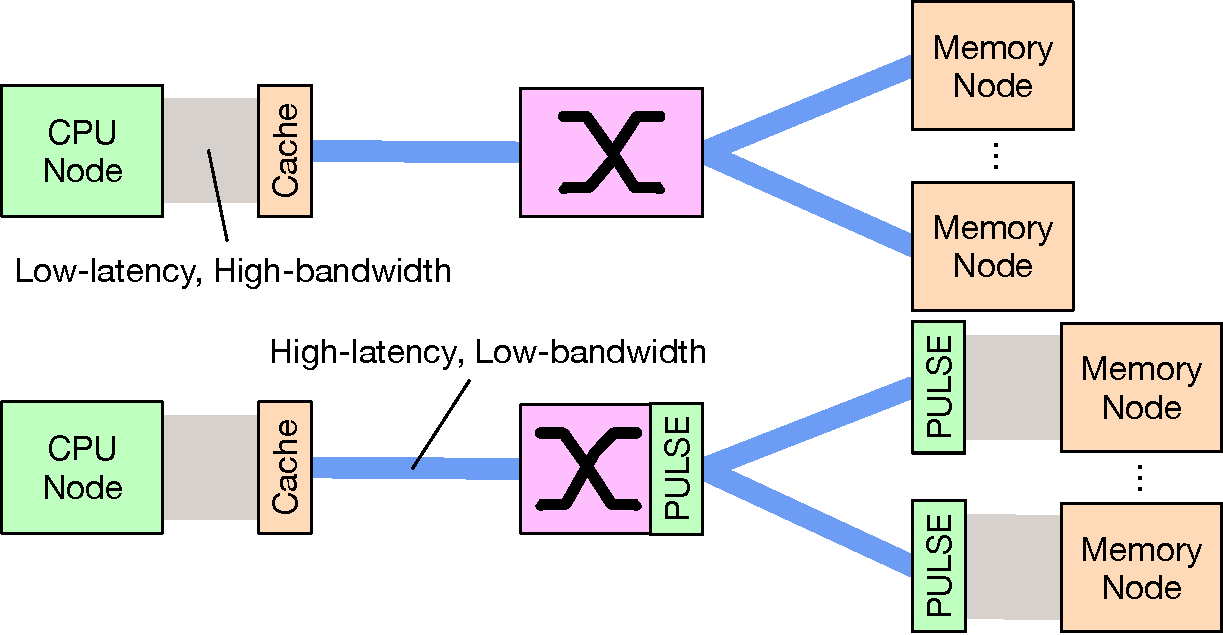
\includegraphics[width=0.98\columnwidth]{fig/pulse/disagg_vertical.pdf}
  \vspace{-0.7em}
  \caption{\textbf{Need for accelerating pointer traversals.} \textit{(top)} The performance of pointer traversals in disaggregated architectures is bottlenecked by slow memory interconnect. \textit{(bottom)} Just as caches offer limited but fast caches near CPUs, we argue that memory needs a counterpart for traversal-heavy workloads: a lightweight but fast accelerator for cache-unfriendly pointer traversals.} 
  \label{fig:disagg}%\vspace{-1.5em}
\end{figure}

\begin{figure*}[ht!]
    \centering
    \subfigure[Our empirical analysis]{
        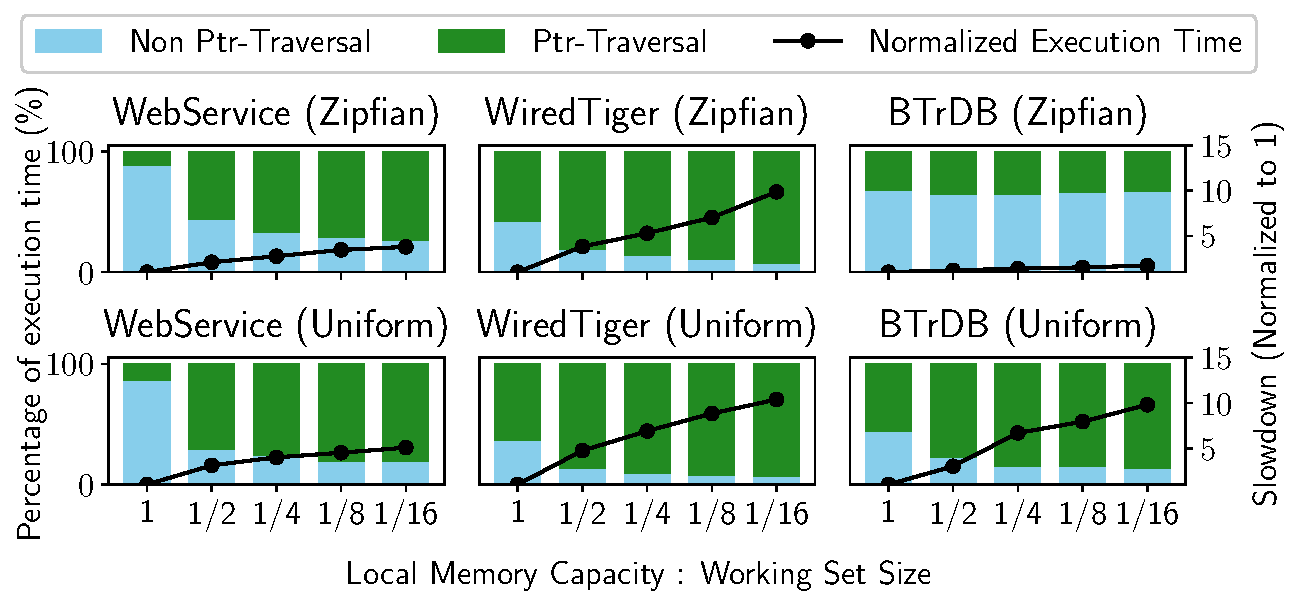
\includegraphics[width=0.40\textwidth]{fig/pulse/figure1_motivation.pdf}
        \label{fig:motivation_experiment}
    }
    \subfigure[\% of distributed traversals]{
        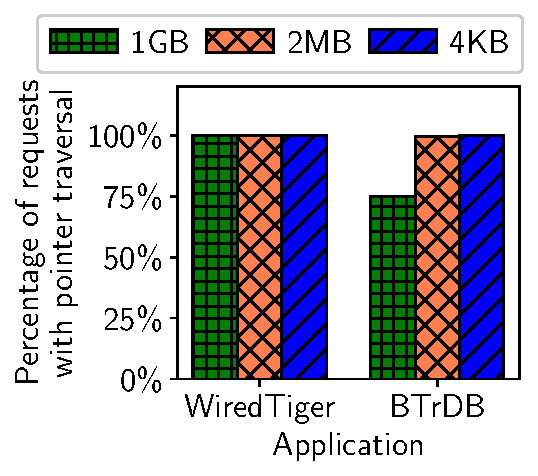
\includegraphics[width=0.21\textwidth]{fig/pulse/distributed.pdf}
        %\vspace{1pt}
        \label{fig:distributed_percentage}
    }
    \subfigure[CDF of distributed traversals]{
        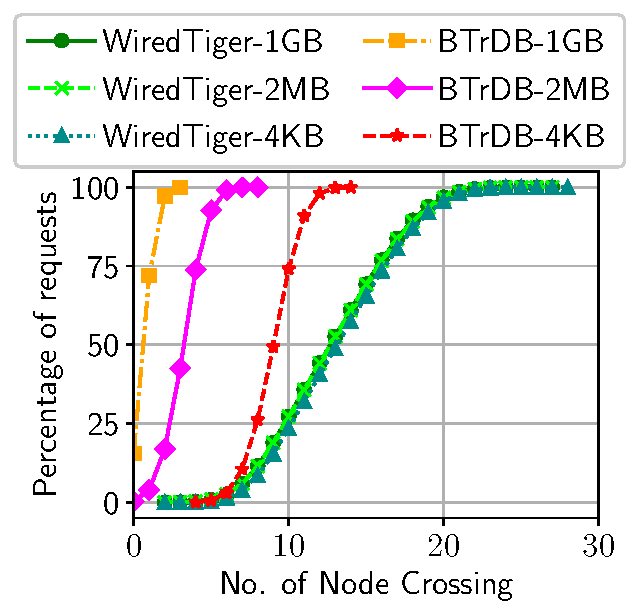
\includegraphics[width=0.24\textwidth]{fig/pulse/cdf.pdf}
        \label{fig:distributed_cdf_wiredtiger}
    }
    \vspace{-1em}
    \caption{\textbf{Time cloud applications spend in pointer traversals.} See \S\ref{ssec:need} for details.} 
    \label{fig:motivation}%\vspace{-1.5em}
\end{figure*}


Similar to how CPUs have small but fast memory (\ie, caches) for quick access to popular data, we argue that memory nodes should also include lightweight but fast processing units with high-bandwidth, low-latency access to memory to speed up pointer-traversals (Fig.~\ref{fig:disagg}~(bottom)). Moreover, the interconnect should facilitate efficient and scalable distributed traversals for deployments with multiple memory nodes that cater to large-scale linked data structures. Prior works have explored systems and API designs for such processing units under multiple settings, ranging from near-memory processing and processing-in-memory approaches~\cite{ahn2015scalable, asghari2016chameleon,  dai2018graphh, schuiki2018scalable, mutlu2019processing, lockerman2020livia, tu2022redcim, devic2022_PIM, wang2022_Nearstream, xie2023mpu, mutlu2022modern, oliveira2022accelerating, eckert2022eidetic, chi2016prime, seshadri2017simple, kwon2019_TensorDIMM, boroumand2019_codna, cho2020_data, ke2020_RecNMP, wang2021stream, xie2021spacea, ke2021near, singh2021fpga, olgun2022pidram, dai2022dimmining, gu2020ipim, gomez2023evaluating, walkers, impica} for single-server architectures, to the use of CPUs~\cite{storagefunctions, splinter, aifm, kayak_nsdi_21, storm_systor_19, zhang2022_teleport} or FPGAs~\cite{clio, strom} near remote/disaggregated memory, but have several key shortcomings. 


% Related work
Specifically, existing approaches are limited in scale and expose a three-way tradeoff between expressiveness, energy efficiency, and performance. First, and perhaps most crucially, none of the existing approaches can accelerate pointer traversals that span \emph{multiple} network-attached memory nodes. 

This limits memory utilization and elasticity since applications must confine their data to a single memory node to accelerate pointer traversals. Their inability to support distributed pointer traversals stems from complex management of address translation state that is required to identify if a traversal can occur locally or must be re-routed to a different memory node (\S\ref{ssec:prior}). Second, existing single-node approaches use full-fledged CPUs for expressive and performant execution of pointer-traversals~\cite{storagefunctions, splinter, aifm, kayak_nsdi_21}. However, coupling large amounts of processing capacity with memory --- which has utility in reducing data movement in PIM architectures~\cite{ahn2015scalable, dai2018graphh, schuiki2018scalable, mutlu2019processing, mutlu2022modern, oliveira2022accelerating, eckert2022eidetic, xie2023mpu, tu2022redcim, lockerman2020livia, asghari2016chameleon, devic2022_PIM, wang2022_Nearstream} ---  goes against the very spirit of memory disaggregation since it leads to poor utilization of compute resources and, consequently, poor energy efficiency. 

Approaches that use wimpy processors at SmartNICs~\cite{rmc_hotnets20, redn} instead of CPUs retain expressiveness, but the limited processing speeds of wimpy nodes curtail their performance and, ultimately lead to lower energy efficiency due to their lengthened executions (\S\ref{ssec:application-study},~\cite{clio}). Lastly, FPGA-based~\cite{clio, strom, sun2023demystifying} and ASIC-based~\cite{impica, walkers} approaches achieve performance and energy efficiency by hard-wiring pointer traversal logic for specific data structures, limiting their expressiveness.  


We design \name\footnote{\textbf{P}rocessing \textbf{U}nit for \textbf{L}inked \textbf{S}tructur\textbf{E}s.}, a distributed pointer-traversal framework for rack-scale disaggregated memory, to meet all of the above needs --- namely, expressiveness, energy efficiency, performance --- via a principled redesign of near-memory processing for disaggregated memory. Central to \name's design is an expressive iterator interface that readily lends itself to a unifying abstraction across most pointer traversals in linked data structures used in key-value stores~\cite{redis, memcached}, databases~\cite{wiredtiger, btree1, btree2, trie1, trie3}, and big-data analytics~\cite{powergraph, graphx, graphchi, pagerank} (\S\ref{sec:interface}). \name's use of this abstraction not only makes it immediately useful in this large family of real-world traversal-heavy use cases, but also enables (i) the use of familiar compiler toolchains to support these use cases with little to no application modifications and (ii) the design of tractable hardware accelerators and efficient distributed traversal mechanisms that exploit properties unique to iterator abstractions.


In particular, \name enables transparent and efficient execution of pointer traversals for our iterator abstraction via a novel accelerator that employs a \emph{disaggregated} architecture to decouple logic and memory pipelines, exploiting the inherently sequential nature of compute and memory accesses in iterator execution (\S\ref{sec:accelerator}). This permits high utilization by provisioning more memory and fewer logic pipelines to cater to memory-centric pointer traversal workloads. A scheduler breaks pointer traversal logic from multiple concurrent workloads across the two sets of pipelines and employs a novel multiplexing strategy to maximize their utilization. While our implementation leverages an FPGA-based SmartNIC due to the high cost and complexity of ASIC fabrication, our ultimate vision is an ASIC-based realization for improved performance and energy efficiency. 

We enable distributed traversals by leveraging the insight that pointer traversal across network-attached memory nodes is equivalent to packet routing at the network switch (\S\ref{sec:distributed}). As such, \name leverages a programmable network switch to inspect the next pointer to be traversed within iterator requests and determine the next memory node to which the request should be forwarded --- both at line rate. We implement a real-system prototype of \name on a disaggregated rack of commodity servers, SmartNICs, and a programmable switch with full-system effects. None of \name's hardware or software changes are invasive or overly complex, ensuring deployability.  Our evaluation of end-to-end real-world workloads shows that \name outperforms disaggregated caching systems with $9$--$34\times$ lower latency and $28$--$171\times$ higher throughput. Moreover, our Xilinx XRT~\cite{xilinx_xrt} and Intel RAPL~\cite{intel_rapl}-based power analysis shows that \name consumes $4.5$--$5\times$ less energy than RPC-based schemes (\S\ref{sec:evaluation}).

\subsection{Motivation and \name Overview}
\label{sec:overview}

\subsubsection{Need for Accelerating Pointer Traversals}
\label{ssec:need}

Memory-intensive applications~\cite{scuba, cachelib, tao, memcache, flighttracker, twittercache, spark} often require traversing linked structures like lists, hash tables, trees, and graphs. 
While disaggregated architectures provide large memory pools across network-attached memory nodes, traversing pointers over the network is still slow~\cite{disagg}. Recent proposals~\cite{disagg, legoos, mind, infiniswap, fastswap} alleviate this slowdown by using the DRAM at the CPU nodes to cache ``hot'' data, but such caches often fare poorly for pointer traversals, as we show next. 

\paragraphb{Pointer traversals in real-world workloads} Prior studies~\cite{graphchi, monetdb, spark, voltdb, memc3, db1000, memcached} have shown that real-world data-centric cloud applications spend anywhere from $21\%$ to $97\%$ of execution time traversing pointers. We empirically analyze the time spent in pointer traversals for three representative cloud applications --- a WebService frontend~\cite{aifm}, indexing on WiredTiger~\cite{wiredtiger}, and time-series analysis on BTrDB~\cite{btrdb} --- with swap-based disaggregated memory~\cite{infiniswap}\footnote{We defer the details of the data structures and workloads employed by these applications, as well as the disaggregated memory setup to \S\ref{sec:evaluation}.}. We vary the cache size at the CPU node from $6.25$\%-$100$\% of each application's working set size. Fig.~\ref{fig:motivation_experiment} shows that (i) all three applications spend a significant fraction of their execution time ($13.6$\%, $63.7$\%, and $55.8$\%, respectively) traversing pointers even when their entire working set is cached, and (ii) the time spent traversing pointers (and thus, the end-to-end execution time) increases with smaller CPU node caches. While the impact of access skew is application-dependent, pointer traversals dominate application execution times when more of the application's working set size is remote. 


\paragraphb{Distributed traversals} As the number of applications and the working-set size per application grows larger, disaggregated architectures must allocate memory across multiple memory nodes to keep up. Such approaches~\cite{legoos, mind, infiniswap, fastswap} tend to strive for the smallest viable allocation granularity with reasonable metadata overheads (e.g., $1$ GB in~\cite{legoos}, $2$ MB in~\cite{mind}) since smaller allocations permit better load balancing and high memory utilization. Unfortunately, finer-grained allocations may cause an application's linked structures to get fragmented across multiple network-attached memory nodes, necessitating many \emph{distributed} traversals. 

Fig.~\ref{fig:distributed_percentage} illustrates this impact on a setup with $1$ compute and $4$ memory nodes: even with large $1$ GB allocations, WiredTiger and BTrDB require over 97\% and 75\% of their requests, respectively, to cross memory node boundaries at least once, with the volume of cross-node traffic increasing at smaller granularities. Fig.~\ref{fig:distributed_cdf_wiredtiger} shows the CDF of requests that require a certain number of memory node crossings. While the randomly ordered data in WiredTiger necessitate many cross-node traversals even for large allocations, the time-ordered data in BTrDB reduce cross-node traversals for larger allocation granularities by confining large time windows to the same memory node. However, smaller to moderate allocation granularities --- required for high memory utilization --- still require many cross-node traversals. 

\subsubsection{Shortcomings of Prior Approaches}
\label{ssec:prior}



No prior work achieves all four properties required for pointer traversals on disaggregated memory: distributed execution, expressiveness, energy efficiency, and performance. We focus on network-attached memory, although a similar analysis extends to in-memory processing~\cite{walkers, ahn2015scalable, impica, asghari2016chameleon, chi2016prime, seshadri2017simple, dai2018graphh, schuiki2018scalable, mutlu2019processing, kwon2019_TensorDIMM, boroumand2019_codna, gu2020ipim, lockerman2020livia, cho2020_data, ke2020_RecNMP, wang2021stream, xie2021spacea, ke2021near, singh2021fpga, olgun2022pidram, mutlu2022modern, oliveira2022accelerating, eckert2022eidetic, tu2022redcim, dai2022dimmining, devic2022_PIM, wang2022_Nearstream, gomez2023evaluating, xie2023mpu}.
 

\paragraphb{No support for distributed execution} Distributed pointer traversals are required to ensure applications can efficiently access large pools of network-attached memory nodes. Unfortunately, to our knowledge, none of the prior works support efficient multi-node pointer traversals. Therefore, applications must confine their data to a single node for efficient traversals, exposing a tradeoff between application performance and scalability. Recent proposals~\cite{sherman, clover, fusee, rolex, marlin, sephash, ditto} explore specialized data structures that co-design partitioning and allocation policies to reduce distributed pointer traversals atop disaggregated memory. Such approaches complement our work since they still require efficient distributed traversals when their optimizations are not applicable, \eg, not many data structures benefit from such specialized co-designs. 

\begin{figure*}[ht!]
  \centering
  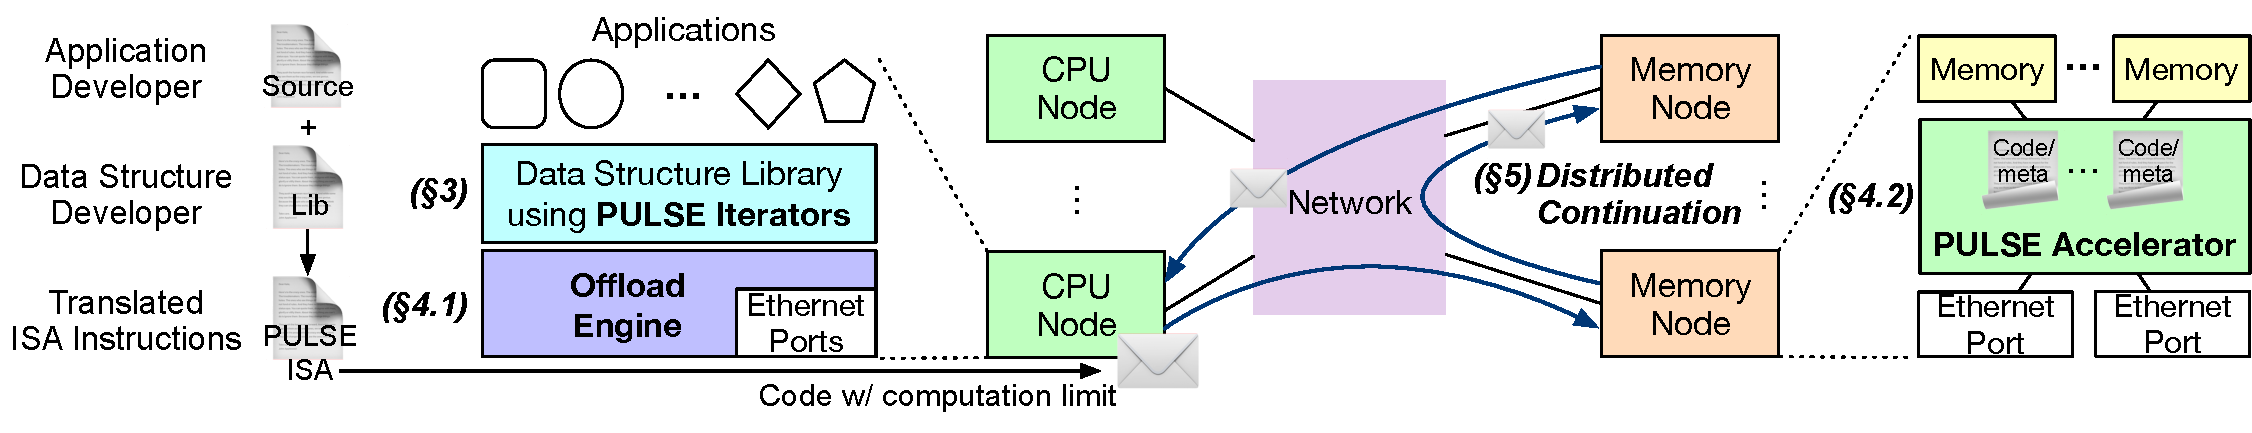
\includegraphics[width=0.85\textwidth]{fig/pulse/overview.pdf}
  \vspace{-1em}
  \caption{\textbf{\name Overview.} Developers use \name's iterator interface (\S\ref{sec:interface}) to express pointer traversals, translated to \name ISA by its dispatch engine (\S\ref{ssec:compute_node}). During execution, \name accelerator ensures energy efficiency (\S\ref{ssec:architecture}) and in-network design enable distributed traversals (\S\ref{sec:distributed}).} 
  \label{fig:general}\vspace{-1em}
\end{figure*}

\paragraphb{Poor utilization/power-efficiency in CPUs} Many prior works have explored remote procedure call (RPC) interfaces to enable offloading computation to CPUs on memory nodes~\cite{aifm, kayak_nsdi_21, splinter, storagefunctions, storm_systor_19}. While CPUs are performant and versatile enough to support most general-purpose computations, the same versatility makes them overkill for pointer traversal workloads in disaggregated architectures --- the CPUs on memory nodes are likely to be underutilized and, consequently, waste energy (\S\ref{sec:evaluation}), since such workloads are memory-intensive and bounded by memory bandwidth rather than CPU cycles. 
Since inefficient power usage resulting from coupled compute and memory resources is the main problem disaggregation aims to resolve, leveraging CPUs at memory nodes essentially nullifies these benefits. 

\paragraphb{Limited expressiveness in FPGA/ASIC accelerators} Another approach explored in recent years uses FPGAs~\cite{clio,strom} or ASICs~\cite{impica, walkers} at memory nodes for performance and energy efficiency. FPGA approaches exploit circuit programmability to realize performant on-path data processing, albeit only for specific data structures, limiting their expressiveness. Although some FPGA approaches aim for greater expressiveness by serving RPCs~\cite{coyote}, RPC logic must be pre-compiled before it is deployed and physically consumes FPGA resources. This limits how many RPCs can be deployed on the FPGA concurrently and also elides runtime resource elasticity for different pointer traversal workloads. ASIC approaches either support a single data structure or provide limited ISA specialized for a single data structure (\eg, linked-lists~\cite{walkers}), limiting their general applicability. 

\paragraphb{Poor performance/power efficiency in wimpy SmartNICs} The emergence of programmable SmartNICs has driven work on offloading computations to the onboard network processors. Some approaches utilize wimpy processors (\eg, ARM or RISC-V processors)~\cite{rmc_hotnets20} or RDMA processing units (PUs)~\cite{redn} to support general-purpose computations near memory. While these wimpy processors can eliminate multiple network round trips in pointer traversal workloads, their processing speeds are far slower than CPU-based or FPGA-based accelerators. Often, such PUs can become a performance bottleneck, especially at high memory bandwidth ($\sim$500 Gbps)~\cite{redn, disagg}. Moreover, wimpy processors tend not to be energy-efficient since their slower execution tends to waste more static power, resulting in higher energy per pointer traversal offload --- an observation noted in prior work~\cite{clio} and confirmed in our evaluation (\S\ref{sec:evaluation}). 


\subsubsection{\name Design Overview}
\label{ssec:overview}


%To achieve the requirements outlined in \S\ref{ssec:need}, 
\name innovates on three key design elements (Fig.~\ref{fig:general}). Central to \name's design is its iterator-based programming model (\S\ref{sec:interface}) that requires minimal effort to port real-world data structure traversals. \name supports \emph{stateful} traversals using a \emph{scratchpad} of pre-configured size, where developers can store and update arbitrary intermediate states (\eg, aggregators, arrays, lists, \etc) during the iterator's execution. Properties specific to iterator patterns enable tractable accelerator design and efficient distributed traversals in \name. 

The iterator code provided by the data structure developer is translated into \name's instruction set architecture (ISA) to be executed by \name accelerators (\S\ref{sec:accelerator}). \name achieves energy efficiency and performance through a novel accelerator that employs disaggregated logic and memory pipelines and an ISA specifically designed for the iterator pattern. Our accelerator employs a scheduler specialized for its disaggregated architecture to ensure high utilization \emph{and} performance. 


\name supports scalable distributed pointer traversals by leveraging programmable network switches to reroute any requests that must cross memory node boundaries (\S\ref{sec:distributed}). \name employs hierarchical address translation \emph{in the network}, where memory node-level address translation is performed at the switch (\ie, a request is routed to the memory node based on its target address), and the memory node accelerator performs translation and protection for local accesses. During traversal, a memory node accelerator can return a request to the switch if it determines the address is not local; the switch re-routes the request to the correct memory node.


\paragraphb{Assumptions} \name does not offload synchronization to its accelerators but instead requires the application logic at the CPU node to explicitly acquire/release appropriate locks for the offloaded operation. Recent efforts enable locking primitives on NICs~\cite{sherman, clover} and programmable switches~\cite{netlock}; these are orthogonal to our work and can be incorporated into \name.d
Finally, \name does not innovate on caching and adapts the caching scheme from prior work~\cite{aifm}, which maintains a transparent cache within the data structure library. 
\section{\name Programming Model}
\label{sec:interface}
\label{ssec:iterators}
\label{ssec:iteratorexample}
We begin with \name's programming model since a carefully crafted interface is crucial to enable wide applicability for real-world traversal-heavy applications, as well as the design of tractable pointer traversal accelerators and efficient distributed traversal mechanisms. \name's interface is intended for data structure library developers to offload pointer traversals in linked data structures. Since \name code modifications are restricted to data structure libraries, existing applications utilizing their interfaces require no modifications. 

We analyzed the implementations of a wide range of popular data structures~\cite{stl, boost, javaiterator, c++iterator} 

to determine the structures common to them in pointer traversals. We found that most traversals (1) initialize a start pointer using data structure-specific logic, (2) iteratively use data structure-specific logic to determine the next pointer to look up, and (3) check a data structure-specific termination condition at the end of each iteration to determine if the traversal should end. 
This structure resembles that of the \emph{iterator} design pattern, establishing its universality as a design motif common to almost all languages~\cite{javaiterator}. This is precisely what makes it an ideal candidate for the interface between the hardware and software layers for pointer traversals. As such, \name allows developers to program their data structure traversals using the iterator interface shown in Listing~\ref{lst:iterator}. 

The interface exposes three functions that must be implemented by the user: (1) \code{init()}, which takes as input arbitrary data structure-specific state to initialize the start pointer, (2) \code{next()}, that updates the current pointer to the next pointer it must traverse to, and, (3) \code{end()}, that determines if the pointer traversal should end (either in success or failure) based on the current pointer. \name then uses the provided implementations for these functions to execute the pointer traversal iteratively, using the \code{execute()} function. We discuss two key novel aspects of our iterator abstraction that were necessary to increase and limit the expressiveness of operations on linked data structures. 

\begin{figure}
\centering
\begin{lstlisting}[caption={\name interface.},label={lst:iterator},escapechar=|]
class pulse_iterator {
    void init(void *) = 0; // Implemented by developer
    void *next() = 0; // Implemented by developer
    bool end() = 0; // Implemented by developer
    
    unsigned char *execute() { // Non-modifiable logic
      unsigned int num_iter = 0;
      while (!end() && num_iter++ < MAX_ITER)
        cur_ptr = next();
      return scratch_pad;|\label{line:scratch_return}|
    }
    uintptr_t cur_ptr;
    unsigned char scratch_pad[MAX_SCRATCHPAD_SIZE];
}
\end{lstlisting}

\end{figure}

\paragraphb{Stateful traversals} Pointer traversals in many data structures are stateful, and the nature of the state can vary widely. For instance, in hash table lookups, the state is the search key that must be compared against a linked list of keys in a hash bucket. In contrast, summing up values across a range of keys in a B-Tree requires maintaining a running variable for storing the sum and updating it for each value encountered in the range. To facilitate this, \name iterators maintain a \code{scratch\_pad} that the developer can use to store an arbitrary state. The state is initialized in \code{init()}, updated in \code{next()}, and finalized in \code{end()}. Since \code{execute()} in \name's iterator interface returns the contents of \code{scratch\_pad} (Line~\ref{line:scratch_return}), developers can place the data that they want to receive in it.


\paragraphb{Bounded computations} \name accelerators support only lightweight processing in memory-intensive operations for high memory bandwidth utilization. While \code{init()} is executed on the CPU node, \code{next()} and \code{end()} are offloaded to \name accelerators; hence, \name limits what memory accesses and computations can be performed in them in two ways. Within each iteration, \name disallows nondeterministic executions, such as unbounded loops, \ie, loops that cannot be unrolled to a fixed number of instructions. 

Across iterations, \code{execute()} in Listing~\ref{lst:iterator} limits the maximum number of iterations that a single request is allowed to perform. This ensures that a particularly long traversal does not block other requests for a long time.  
If a request exceeds the maximum iteration count, \name terminates the traversal and returns the \code{scratch\_pad} value to the CPU node, which can issue a new request to continue the traversal from that point. 

\begin{figure}[t]
\centering
% \vspace{-5pt}
\begin{lstlisting}[caption={C++ STL realization for \code{unordered\_map::find()}.},label={lst:stl}]
struct node {
  key_type key;
  value_type value;
  struct node *next;
};

value_type find(key_type key) {
  for (struct node *cur_ptr = bucket_ptr(hash(key)); ; cur_ptr = cur_ptr->next) {
    if (key == cur_ptr->key) // Key found
      return cur_ptr->value;
    if (cur_ptr->next == nullptr) // Key not found
      break;
  }
  return KEY_NOT_FOUND;
}
\end{lstlisting}
\begin{lstlisting}[caption={\name realization for \code{unordered\_map::find()}.},label={lst:stl_mod}]
class unordered_map_find : pulse_iterator {
  init(void *key) {
    memcpy(scratch_pad, key, sizeof(key_type));
    cur_ptr = bucket_ptr(hash((key_type)*key));
  }
  
  void* next() { return cur_ptr->next; }
  
  bool end() {
    key_type key = *((key_type *)scratch_pad);
    if (key == cur_ptr->key) { // Key found
      *((value_type *)scratch_pad) = cur_ptr->value;
      return true;
    }
    if (cur_ptr->next == nullptr) { // Key not found
      *((unsigned int *)scratch_pad) = KEY_NOT_FOUND;  
      return true;
    }
    return false;
  }
}
\end{lstlisting}
\end{figure}

\paragraphb{An illustrative example} We demonstrate how the \code{find()} operation on C++ STL \code{unordered\_map} can be ported to \name. Listing~\ref{lst:stl} shows a simplified version of its implementation in STL --- the pointer traversal begins by computing a hash function and determining a pointer to the hash bucket corresponding to the hash. It then iterates through a linked list corresponding to the hash bucket, terminating if the key is found or the linked list ends without it being found.

Listing~\ref{lst:stl_mod} shows the corresponding iterator implementation in \name. Much of the implementation is unchanged, with minor restructuring for \code{init()}, \code{next()}, and \code{end()} functions. The main changes are --- how the state (the search key) is exchanged across the three functions and how the data is returned back to the user via the \code{scratch\_pad} (an error message if the key is not found, or its value if it is).   


\subsection{Accelerating Pointer Traversals on a Node}
\label{sec:accelerator}


\subsubsection{\name Dispatch Engine}\label{ssec:compute_node}
The dispatch engine is a software framework running at the CPU node for two purposes.  First, it translates the iterator realization for pointer traversal provided by a data structure library developer (\S\ref{sec:interface}) into \name's ISA. Second, it determines if the accelerator can support the computations performed during the traversal, and if so, ships a request to the accelerator at the memory node. If not, the execution proceeds at the CPU node with regular remote memory accesses.

\paragraphb{Translating iterator code to \name ISA} To be readily implementable, \name plugs into existing compiler toolchains. The dispatch engine generates \name ISA instructions using widely known compiler techniques~\cite{llvm}. 
\name's ISA is a stripped-down RISC ISA, only containing operations necessary for basic processing and memory accesses to enable a simple and energy-efficient accelerator design (Table~\ref{tab:isa}). There are, however, a few notable aspects to our adapted ISA and the translation of iterator code to it. First, as noted in \S\ref{ssec:iterators}, \name does not support unbounded loops within a single iteration, \ie, the ISA only supports conditional jumps to points ahead in code. This is similar to eBPF programs~\cite{ebpfjump}, where only forward jumps are supported to prevent the program from running infinitely within the kernel. A backward jump can only occur when the next iteration starts; \name employs a special \code{NEXT\_ITER} instruction to explicitly mark this point so that the accelerator can begin scheduling the memory pipeline (\S\ref{ssec:architecture}). Second, again as noted in \S\ref{ssec:iterators}, developers can maintain state and return values using a \code{scratch\_pad} of pre-configured size; our ISA supports register operations directly on the \code{scratch\_pad} and provides special \code{RETURN} instruction that simply terminates the iterator execution and yields the contents of the \code{scratch\_pad} as the return value. 

Finally, we found that the iterator traversal pattern typically can be broken down into two types of computation --- fetching data\footnote{While the rest of the section focuses only on describing data fetches from memory, we note that writing data to memory proceeds similarly.} pointed to by \code{cur\_ptr} from memory, and processing the fetched data to determine what the next pointer should be, or if the iterator execution should terminate. If the translation from the iterator code to \name's ISA is done naively, it can result in multiple unnecessary loads within the vicinity of the memory location pointed to by \code{cur\_ptr}. For instance, the \code{unordered\_map::find()} realization shown in Listing~\ref{lst:stl_mod} makes references to \code{cur\_ptr->key}, \code{cur\_ptr->value} and \code{cur\_ptr->next} at various points, and if each incurs a separate load, it will slow down execution and waste memory bandwidth. Consequently, \name's dispatch engine \emph{infers} the range of memory locations accessed relative to \code{cur\_ptr} in the \code{next()} and \code{end()} functions via static analysis and aggregates these accesses into a single large \code{LOAD} (of up to 256 B) at the beginning of each iteration. 

% \begin{figure*}
\begin{table}[btp!]
    %\vspace{2pt}
    \centering
    \footnotesize  % 8 pt for 10 pt body (small for 9pt)
    \def\arraystretch{0.98}%
    % \footnotesize % 8 pt for 10 pt body
    % \resizebox{0.475\textwidth}{!}{
    \begin{tabular}{l|l|l}
      \hline
      \textbf{Class}  & \textbf{Instructions} & \textbf{Description}\\\hline\hline
      Memory  & \smallcode{LOAD}, \smallcode{STORE} & \specialcell{Load/store data\\ from/to address.} \\  \hline
      ALU & \specialcell{\smallcode{ADD}, \smallcode{SUB}, \smallcode{MUL}, \smallcode{DIV},\\ \smallcode{AND}, \smallcode{OR}, \smallcode{NOT}} & Standard ALU operations. \\ \hline
      Register & \smallcode{MOVE} & Move data b/w registers.\\ \hline
      Branch  & \specialcell{\smallcode{COMPARE} and\\ \smallcode{JUMP\_}\{\smallcode{EQ}, \smallcode{NEQ}, \smallcode{LT}, ...\}} & \specialcell{Compare values \& jump\\ ahead based on condition\\ (\eg, equal, less than, \etc).}\\ \hline
      Terminal & \smallcode{RETURN}, \smallcode{NEXT\_ITER} & \specialcell{End traversal \& return,\\ or start next iteration.} \\
     \hline\hline
    \end{tabular}
    % }%\vspace{-.5em}
    \caption{\textbf{\name adapts a restricted subset of RISC-V ISA} (\S\ref{ssec:compute_node}).}
    \label{tab:isa}
    % \vspace{-1.5em}
\end{table}
% \end{figure*}


\paragraphb{Bounding complexity of offloaded code} While \name's interface and ISA already limit the \emph{types} of computation than can be performed per iteration, \name also needs to limit the \emph{amount} of computation per iteration to ensure the operations offloaded to \name accelerators remain memory-centric. To this end, \name's dispatch engine analyzes the generated ISA for the iterator to determine the time required to execute computational logic ($t_c$) and the time required to perform the single data load at the beginning of the iteration ($t_d$).

\name exploits the known execution time of its accelerators in terms of time per compute instruction, $t_i$, to determine $t_c = t_i \cdot N$, where $N$ is the number of instructions per iteration. The CPU node offloads the iterator execution only if $t_c \leq \eta \cdot t_d$, where $\eta$ is a predefined accelerator-specific threshold. Note that since we only want to offload memory-centric operations, $\eta \leq 1$. As we will show in \S\ref{ssec:architecture}, the choice of $\eta$ allows \name to maximize the memory bandwidth utilization and ensure processing never becomes a bottleneck for pointer traversals.


\paragraphb{Issuing network requests to accelerator} Once the dispatch engine decides to offload an iterator execution, it encapsulates the ISA instructions (\code{code}) along with the initial value of \code{cur\_ptr} and \code{scratch\_pad} (initialized by \code{init()}) into a network request. It issues the request, leaving the network to determine which memory node it should be forwarded to (\S\ref{sec:distributed}). To recover from packet drops, the dispatch engine embeds a request identifier (ID) with the CPU node ID and a local request counter in the request packets, maintains a timer per request, and retransmits requests on timeout.

\paragraphb{Practical deployability} Our software stack is readily deployable due to its use of real-world toolchains. Our user library adapts implementations of common data structures used in key-value stores~\cite{redis, memcached}, databases~\cite{wiredtiger, btree1, btree2, trie1, trie3}, and big-data analytics~\cite{powergraph, graphx, graphchi, pagerank} to \name's iterator interface (\S\ref{sec:interface}). \name's dispatch engine is implemented on Intel DPDK-based~\cite{dpdk} low-latency, high-throughput UDP stack. \name compiler adapts the Sparc backend of LLVM~\cite{llvmsparc} since its ISA is close to \name's ISA. Our LLVM frontend applies a set of analysis and optimization passes~\cite{llvmpass} to enforce \name constraints and semantics: the analysis pass identifies code snippets that require offloading, while the optimization pass translates pointer traversal code to \name ISA.


% !TEX root = ../paper.tex
\subsubsection{\name Accelerator Design}
\label{ssec:architecture}
\label{ssec:traversalexample}
% Partitioning operation into memory and processing
The accelerator is at the heart of \name design and is key to ensuring high performance for iterator executions with high resource and energy efficiency. Our motivation for a new accelerator design stems from two unique properties of iterator executions on linked structures: 



\begin{itemize}[leftmargin=*, itemsep=0pt]
  \item \textbf{Property 1:} Each iteration involves two clearly separated but sequentially dependent steps: (i) fetching data from memory via a pointer (\eg, a list or tree node), followed by (ii) executing logic on the fetched data to identify the next pointer. The logic cannot be executed concurrently with or before the data fetch, and the next data fetch cannot be performed until the logic execution yields the next pointer.
 
  \item \textbf{Property 2:} Iterators that benefit from offload spend more time in data fetch ($t_d$) than logic execution ($t_c$), \ie, $t_c < \eta \cdot t_d$, where $\eta \leq 1$, as noted in \S\ref{ssec:compute_node}. 
\end{itemize}
\noindent
Any accelerator for iterator executions must have a \emph{memory pipeline} and a \emph{logic pipeline} to support the execution steps (i) and (ii) above. 
The strict dependency between the steps (Property 1) renders many optimizations of traditional multi-core processors, such as out-of-order execution, ineffective. Moreover, since each core in such architectures has tightly coupled logic and memory pipelines, the memory-intensive nature of iterators (Property 2) results in the logic pipeline remaining idle most of the time. These two factors combined result in poor utilization and energy efficiency for such architectures. Fig.~\ref{fig:architecture_overview}~(top) captures this through the execution of 3 iterators (A, B, C), each with $2$ iterations (\eg, A1, A2, etc.), on a multi-core architecture. Since each iteration comprises a data fetch followed by a dependent logic execution, one of the pipelines remains idle while the other is busy. While thread-level parallelism permits iterator requests to be spread across multiple cores for increased overall throughput, per-core under-utilization of logic and memory pipelines persists, resulting in suboptimal resource and energy usage.



\begin{figure}[t]
  \centering
  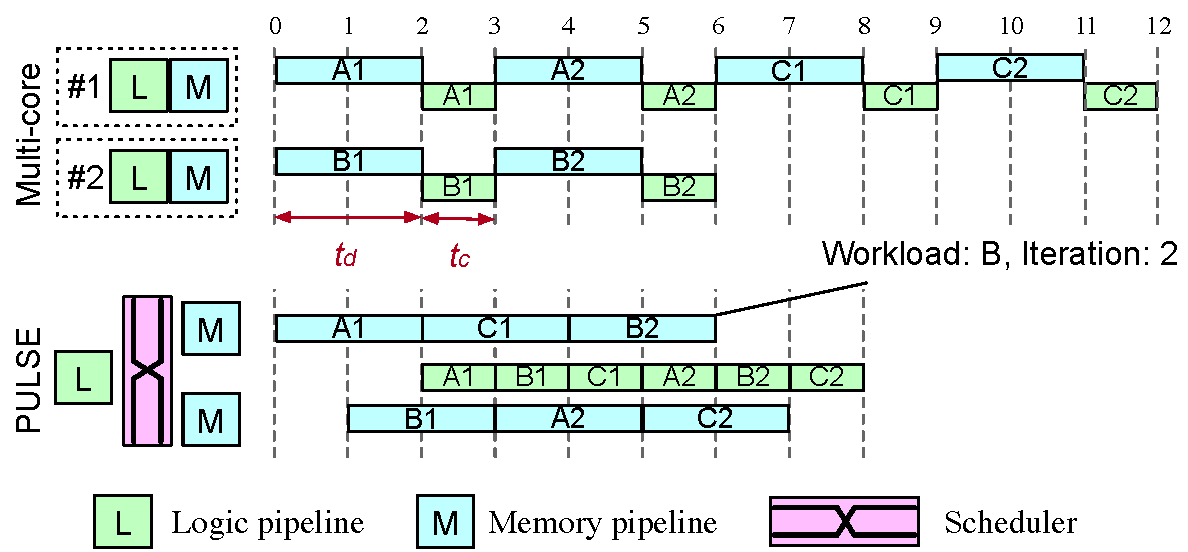
\includegraphics[width=0.9\columnwidth]{fig/pulse/architecture.pdf}
  \vspace{-0.5em}
  \caption{\textbf{\name accelerator architecture.} (top) Traditional multi-core architectures with tightly coupled logic and memory pipelines result in low utilization and longer execution times. (bottom) \name accelerator's \emph{disaggregated} design with an unequal number of logic and memory pipelines efficiently multiplexes concurrent iterator executions across them for near-optimal utilization and performance.}
  \label{fig:architecture_overview}%\vspace{-1.5em}
\end{figure} 

\paragraphb{Disaggregated accelerator design} Motivated by the unique properties of iterators, we propose a novel accelerator architecture that \emph{disaggregates memory and logic pipelines}, using a scheduler to multiplex corresponding components of iterators across them. First, such a decoupling permits an asymmetric number of logic and memory pipelines to maximize the utilization of either pipeline, in stark contrast to the tight coupling in multi-core architectures. In our design, if there are $m$ logic and $n$ memory pipelines, then the accelerator-specific threshold $\eta < 1$ we alluded to in  \S\ref{ssec:compute_node} is $\frac{m}{n}$, \ie, there are fewer logic pipelines than memory pipelines in keeping with Property 2. Fig.~\ref{fig:architecture_overview}~(bottom) shows an example of our disaggregated accelerator design with one logic pipeline and two memory pipelines (\ie, $m=1, n=2$). 

Even though data fetch and logic execution within each iterator must be sequential, the disaggregated design permits efficient multiplexing of data fetch and logic execution from different iterators across the disaggregated logic and memory pipelines to maximize utilization. To see how, recall that the logic execution time $t_c$ for each offloaded iterator execution in \name is $\leq\eta\cdot t_d$, where $t_d$ is its data fetch time (\S\ref{ssec:compute_node}). Consider the extreme case where $t_c=\eta \cdot t_d$ for all offloaded iterator executions --- in this case, it is always possible to multiplex $m+n$ concurrent iterator executions to fully utilize all $m$ logic and $n$ memory pipelines. While we omit a theoretical proof for brevity, Fig.~\ref{fig:architecture_overview}~(bottom) illustrates the multiplexed execution --- orchestrated by a scheduler in our accelerator --- for $t_c=\frac{1}{2}\cdot t_d$ with $3$ iterators. This is the ideal case --- similar multiplexing is still possible if $t_c\leq\eta\cdot t_d$ with complete utilization of memory pipelines, albeit with lower utilization of logic pipelines (since they will be idle for $\frac{t_c - \eta\cdot t_d}{t_c}$ fraction of time). As such, we provision $\eta=\frac{m}{n}$ to be as close to the expected $\frac{t_c}{t_d}$ for the workload to maximize the utilization of logic pipelines. It is possible to improve the logic pipelines' energy efficiency by dynamically down-scaling frequency~\cite{daepowerscaling}; we leave such optimizations to future work.

While the memory pipeline is stateless, the logic pipeline must maintain the state for the iterator it executes. To multiplex several iterator executions, logic pipelines need efficient mechanisms for efficient context switching. To this end, we maintain a dedicated \emph{workspace} corresponding to each iterator's execution. Each workspace stores three distinct pieces of state: \code{cur\_ptr} and \code{scratch\_pad} to track the iterator state described in \S\ref{ssec:iterators}, and \code{data}, which holds the data loaded from memory for \code{cur\_ptr}. A dedicated workspace per iterator allows the logic pipeline to switch to any iterator's execution without delay when triggered by the scheduler, although it requires maintaining multiple workspaces --- a maximum of $m+n$ to accommodate any possible schedule due to our bound on the number of concurrent iterators. We divide these workspaces equally across logic pipelines.


\begin{figure}[t]
\centering
 %\vspace{-0.2em}
  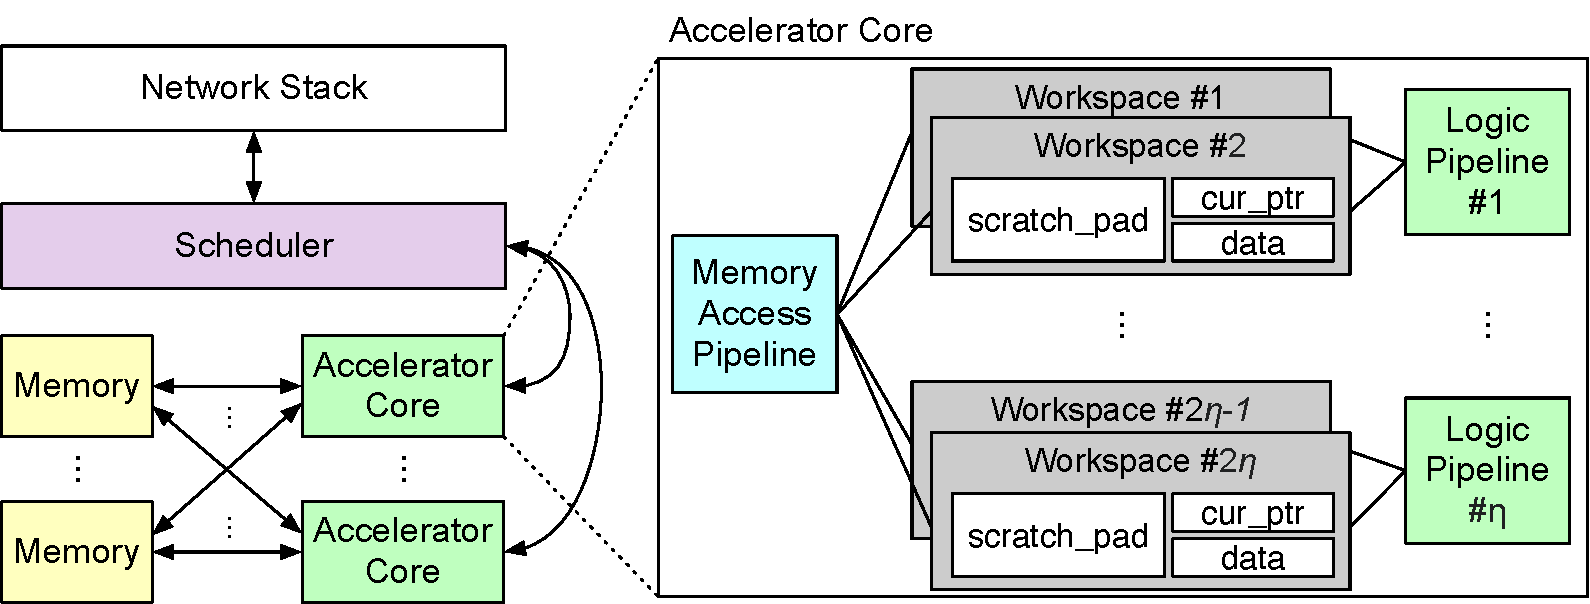
\includegraphics[width=\columnwidth]{fig/pulse/accelerator.pdf}
  \vspace{-2em}
 \caption{\textbf{\name accelerator overview.} See \S\ref{ssec:architecture} for details.}
\label{fig:accelnew}
%\vspace{-2.0em}
\end{figure}

\paragraphb{\name Accelerator Components} \name accelerator comprises $n$ memory and $m$ logic pipelines for executing iterator requests, a scheduler that multiplexes requests across the logic and memory pipelines, and a network stack for parsing pointer-traversal requests from the network (Fig.~\ref{fig:accelnew}).

\paragraphc{Memory pipeline:} Each memory pipeline loads data from the attached DRAM 
to the corresponding workspace assigned by the scheduler at the start of each iteration. This involves (i) address translation and (ii) memory protection based on page access permissions. We realize range-based address translations (simulated in prior work~\cite{range}) in our real-world implementation using TCAM to reduce on-chip storage usage. 

Once a memory access is complete, the memory pipeline signals the scheduler to continue the iterator execution or terminate it if there is a translation or protection failure.


\paragraphc{Logic pipeline:} Each logic pipeline runs \name ISA instructions other than \code{LOAD}/\code{STORE} to determine the \code{cur\_ptr} value for the next iteration or, to determine if the termination condition has been met. Our logic pipeline comprises an ALU to execute the standard arithmetic and logic instructions, as well as modules to support register manipulation, branching, and the specialized \code{RETURN} instruction execution (Table~\ref{tab:isa}). During a particular iterator's execution, the logic pipeline performs its corresponding instructions with direct reads and updates to its dedicated workspace registers. An iteration's logic can end in one of two possible ways: (i) the \code{cur\_ptr} has been updated to the next pointer, and the \code{NEXT\_ITER} instruction is reached, or (ii) the pointer traversal is complete, and the \code{RETURN} instruction is reached. In either case, the logic pipeline notifies the scheduler with the appropriate signal.

\paragraphc{Scheduler:} The scheduler handles new iterator requests received over the network and schedules each iterator's data fetch and logic execution across memory and logic pipelines: 
\begin{enumerate}[leftmargin=*, itemsep=0pt]
  \item On receiving a new request over the network, it assigns the iterator an empty workspace at a logic pipeline and signals one of the memory pipelines to execute the data fetch from memory based on the state in the workspace.\label{signal:1}
  \item On receiving a signal from the memory pipeline that a data fetch has successfully completed, it notifies the appropriate logic pipeline to continue iterator execution via the corresponding workspace.
  \item On receiving a signal from the logic pipeline that the next iteration can be started (via the \code{NEXT\_ITER} instruction), it notifies one of the memory pipelines to execute \code{LOAD} via the corresponding workspace.\label{signal:2}
  \item When it receives a signal from the memory pipeline that an address translation or memory protection failed or a signal from the logic pipeline that the iterator execution has met its terminal condition (via the \code{RETURN} instruction), it signals the network stack to prepare a response containing the iterator \code{code}, \code{cur\_ptr} and \code{scratch\_pad}.
\end{enumerate}
\noindent
While the scheduler assigns memory and logic pipelines to an iterator in steps~\ref{signal:1} and~\ref{signal:2} in a manner that maximizes utilization of all memory pipelines (\ie, Fig.~\ref{fig:architecture_overview}~(bottom)), it is possible to implement other scheduling policies.


\paragraphc{Network Stack:} The network stack receives and transmits packets; when a new request arrives, it parses/deparses the payload to extract/embed the request ID, \code{code}, and state for the offloaded iterator execution (\code{cur\_ptr}, \code{scratch\_pad}). 

The network stack uses the same format for both requests and responses, so a response can be sent back to the CPU node on traversal completion or rerouted as a request to a different memory node for continued execution (\S\ref{sec:distributed}).


\begin{comment}
\begin{figure}[!t]
\begin{lstlisting}[caption={Simplified \name ISA for \code{unordered\_map::find()}.},label={lst:asm},escapechar=|]
Iter_Start:
    /* Load the current node data pointed by cur_ptr */
    LOAD data|\label{line:asm_load_data}|
    /* Target key at offset=0; current key at offset=0 */
    COMPARE scratch_pad[0] data[0]|\label{line:asm_start_compute}|
    /* Forward jump if the key is found */
    JUMP_EQ Return_success
    /* Check the next pointer stored in data at offset=40 */
    COMPARE 0 data[40]
    /* Return; the key was not found */
    JUMP_EQ Return_fail
    /* Set the next pointer at cur_ptr */
    MOVE cur_ptr data[40]
    /* Start the next iteration */
    NEXT_ITER|\label{line:back_jump}|
Return_fail:
    /* Store the result, KEY_NOT_FOUND */
    MOVE scratch_pad[8] KEY_NOT_FOUND
    /* Terminate the loop */
    RETURN
Return_success:
    /* The found data is located in data at offset=8 */
    MOVE scratch_pad[8] data[8]
    /* Terminate the loop */
    RETURN
\end{lstlisting}
%\vspace{-3em}
\end{figure}
\end{comment}


\paragraphb{Implementation} We use an FPGA-based NIC (Xilinx Alveo U250) with two 100 Gbps ports, 64 GB on-board DRAM, 1,728K LUTs, and 70 MB BRAM. Since the board has two Ethernet ports and four memory channels, we partition its resources into two \name accelerators, each with a single Ethernet port and two memory channels. Our analysis of common data structures (\S\ref{sec:evaluation}) shows their $t_c/t_d$ ratio tends to be $<0.75$. As such, we set $\eta=0.75$, \ie, there are four memory and three logic pipelines and a total of $7$ workspaces on the accelerator.
We use the Xilinx TCAM IP~\cite{tcam_ip} (for page tables), $100$ Gbps Ethernet IP, link-layer IPs~\cite{xilinx_network}, and burst data transfers~\cite{burstdatatransfer} to improve memory bandwidth. The logic and memory pipelines are clocked at 250 MHz, while the network stack operates at 322 MHz for 100 Gbps traffic. Our FPGA prototype showcases \name's potential; we believe that ASIC implementations are the next natural step. 



\section{Distributed Pointer Traversals}
\label{sec:distributed}


By restricting pointer traversals to a single memory node (\S\ref{sec:overview}), prior approaches leave applications with two undesirable options. At one extreme, they can confine their data to a single memory, but sacrifice application scalability. Conversely, they can spread their data across multiple nodes but have to return the CPU node whenever the traversal accesses a pointer on another memory node. This affords scalability but costs additional network and software processing latency at the CPU node. To avoid the cost, one may replicate the entire translation and protection state for the cluster at every memory node so they can directly forward traversal requests to other memory nodes. This comes at the cost of increased space consumption for translation, which is challenging to contain within the accelerator's translation and protection tables. Moreover, duplicating this state across memory nodes requires complex protocols for ensuring their consistency (\eg, when the state changes), which have significant performance overheads.

\begin{figure}[t]
\centering
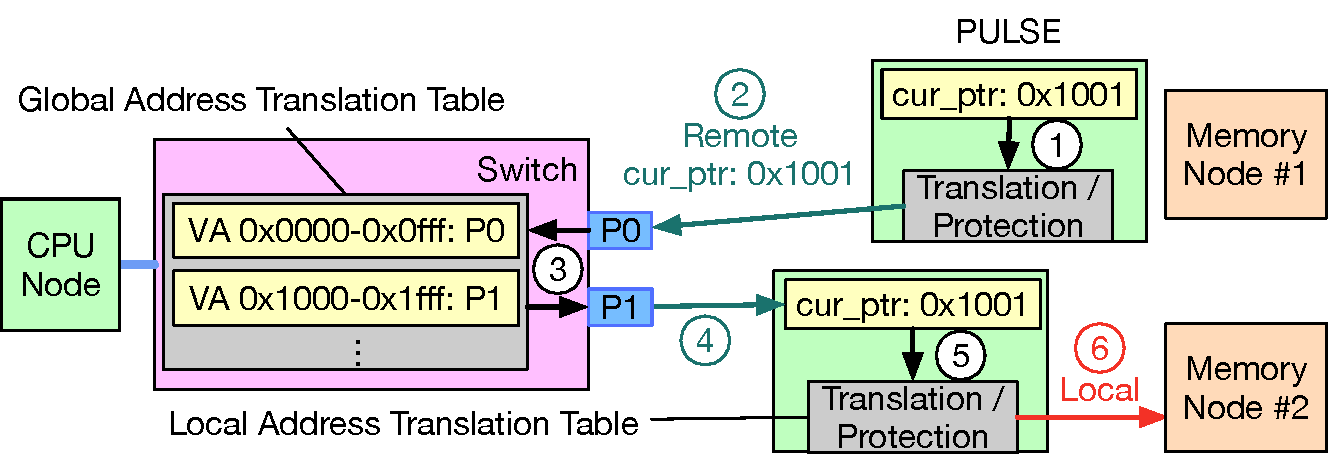
\includegraphics[width=0.96\columnwidth]{fig/pulse/hierarchical.pdf}
\vspace{-1.4em}
\caption{\textbf{Hierarchical translation \& distributed traversal (\S\ref{sec:distributed}).}}
% If local translation fails (\textcircled{1}), \name forwards the request to the switch (\textcircled{2}), which uses the \code{cur\_ptr} field and its global translations (\textcircled{3}) to route it to the appropriate memory node (\textcircled{4}-\textcircled{6}).
\label{fig:hierarchical}%\vspace{-1em}
\end{figure}

\name breaks this tradeoff between performance and scalability by leveraging a programmable network switch to support rack-scale distributed pointer traversals. In particular, if the \name accelerator on one memory node detects that the next pointer lies on a different memory node, it forwards the request to the network switch, which routes it to the appropriate memory node for continuing the traversal. This cuts the network latency by half a round trip time and avoids software overheads at the CPU node, instead performing the routing logic in switch hardware. Since continuing the traversal across memory nodes is similar to packet routing, the switch hardware is already optimized to support it.

Enabling rack-scale pointer traversals, however, requires addressing two key challenges, as we discuss next.

\paragraphb{Hierarchical translation} For the switch to forward the pointer traversal request to the appropriate memory node, it must be able to locate which memory nodes are responsible for which addresses. To minimize the logic and state maintained at the switch due to its limited resources, \name employs hierarchical address translation as shown in Fig.~\ref{fig:hierarchical}. 
In particular, the address space is range partitioned across memory nodes; \name only stores the base address to memory node mapping at the switch, while each memory node stores its own local address translation and protection metadata at the accelerator (\textcircled{1}), as outlined in \S\ref{sec:accelerator}. The routing logic at the switch inspects the \code{cur\_ptr} field in the request (\textcircled{2}) and consults its mapping to determine the target memory node (\textcircled{3}). At the memory node, the traversal proceeds until the accessed pointer is not present in the local table (as in \textcircled{1}); it then sends the request back to the switch (\S\ref{ssec:architecture}), which can re-route the request to the appropriate memory node (\textcircled{4}-\textcircled{6}), or notify the CPU node if the pointer is invalid.
% \slee{I am a bit confused by the next sentence; if the switch think the address is backed by this memory node, there shouldn't be a case where another memory node actually serves it?} 

\paragraphb{Continuing stateful iterator execution} One challenge of distributing iterator execution in \name lies in its stateful nature: since \name permits the storage of intermediate state in the iterator's \code{scratch\_pad}, how can such stateful iterator execution be continued on a different memory node? Fortunately, our design choices of confining all of the iterator state in \code{scratch\_pad} and \code{cur\_ptr} and keeping the request and response formats identical make this straightforward. The accelerator at the memory node simply embeds the up-to-date \code{scratch\_pad} within the response before forwarding it to the switch; when the switch forwards it to the next memory node, it can simply continue execution exactly as it would have if the last memory node had the pointer. 




\begin{figure*}[t]
\centering
  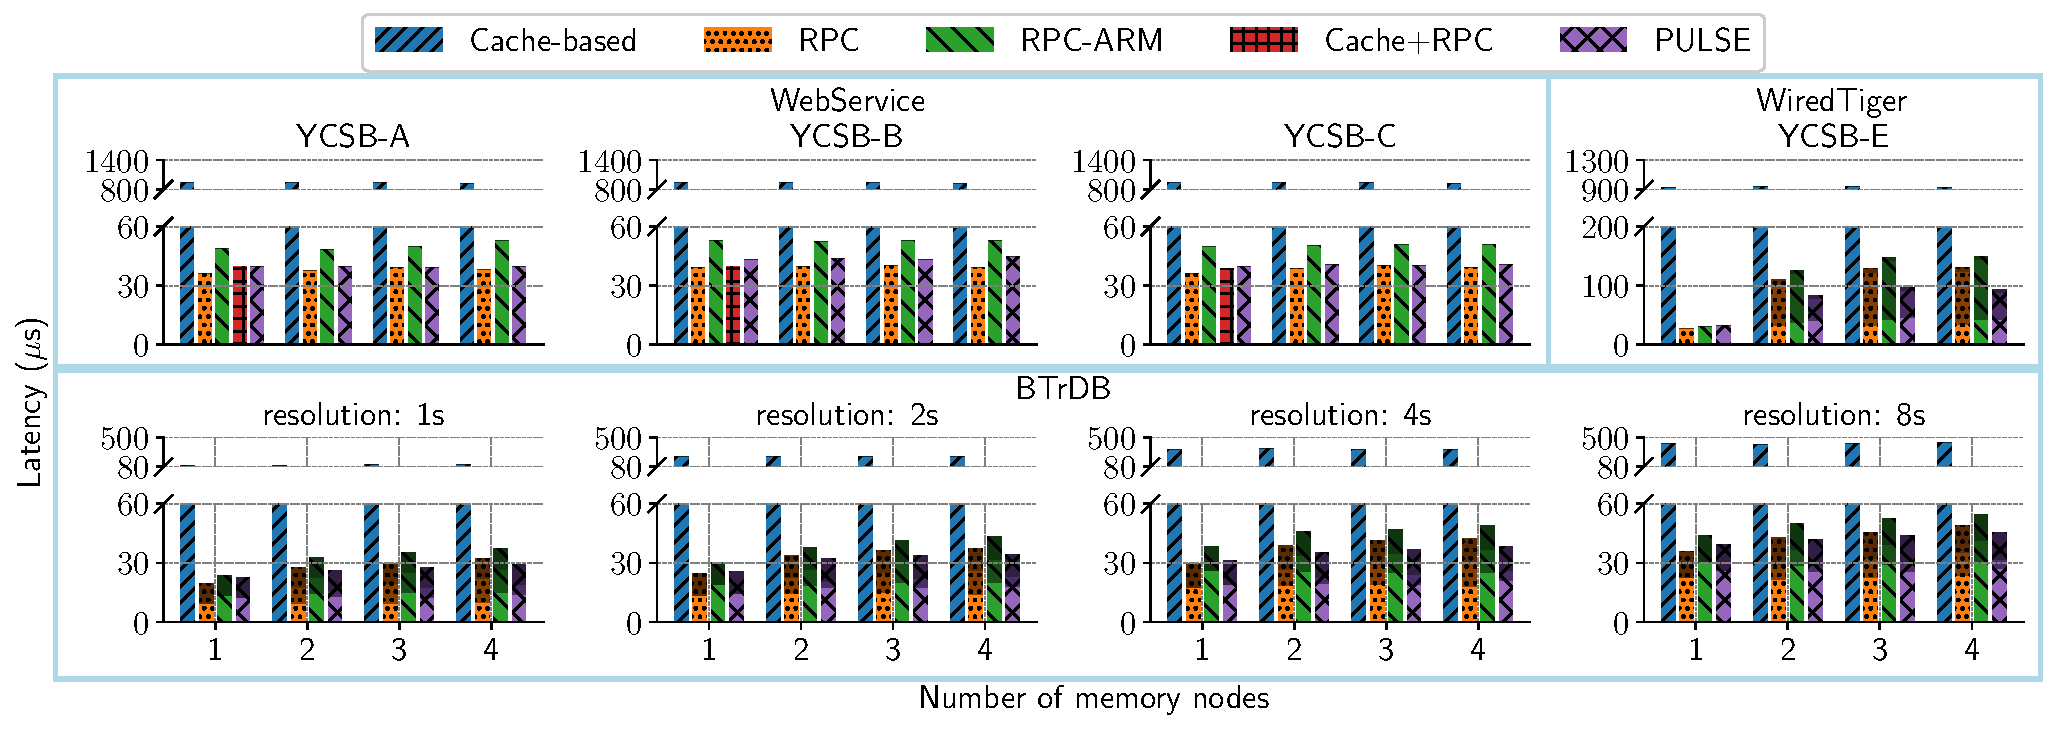
\includegraphics[width=0.8\textwidth]{fig/pulse/latency.pdf}
  \\
  %\vspace{-.5em}
  % \newline
  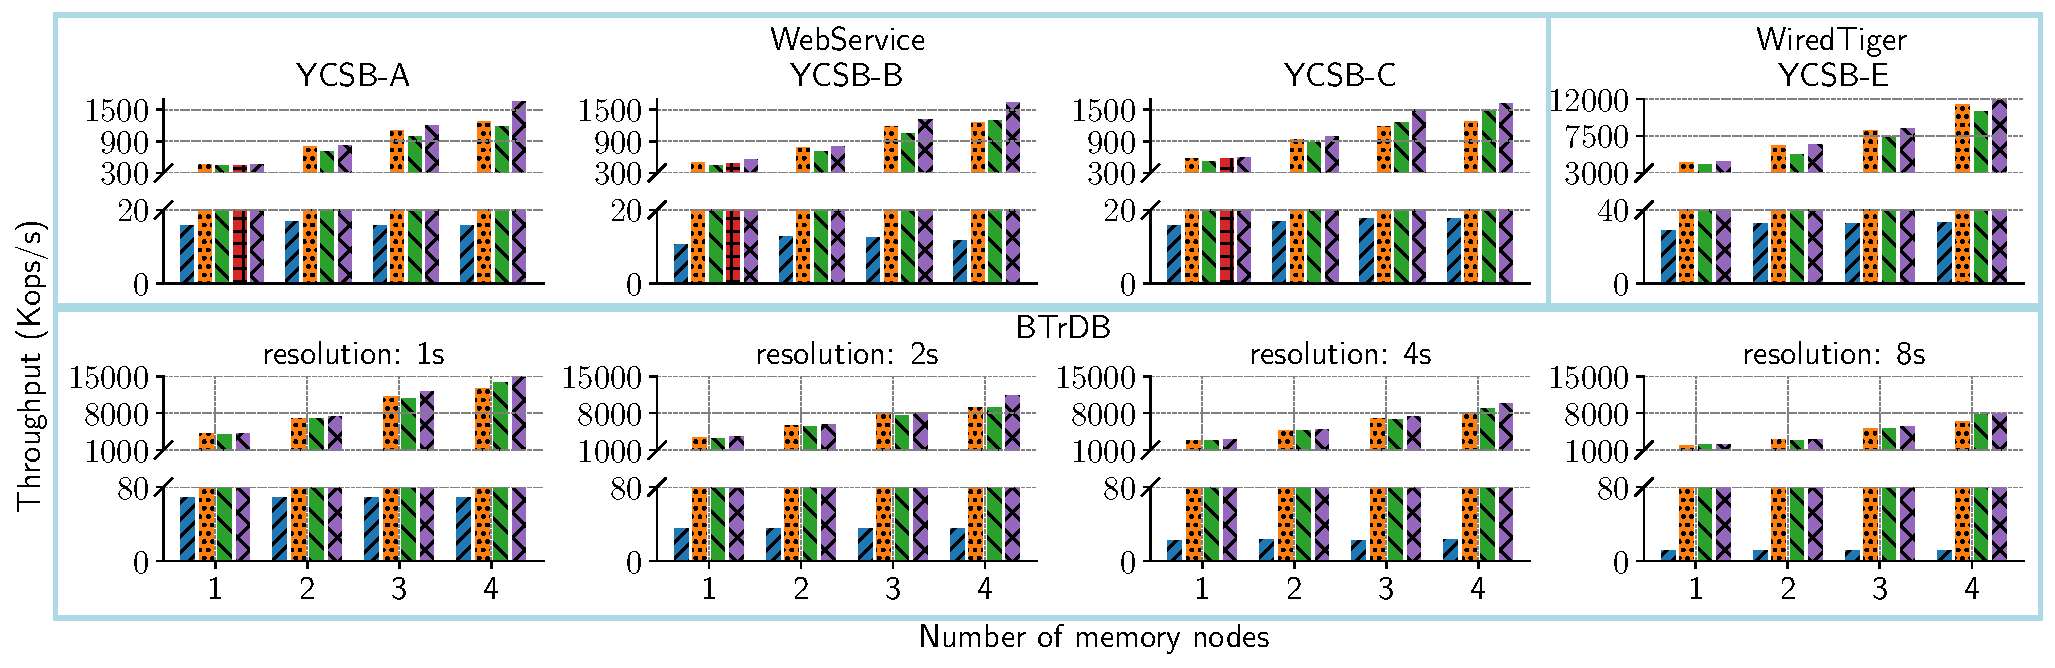
\includegraphics[width=0.8\textwidth]{fig/pulse/throughput.pdf}
  % \\
  \vspace{-1.3em}
  %\vspace{-1em}
  \caption{\textbf{Application latency (top) \& throughput (bottom) (\S\ref{ssec:application-study}).} 
  The darker color indicates the time spent on cross-node pointer traversals, which increases with the number of memory nodes in WiredTiger and BTrDB.}
\label{fig:eval_perf_e2e_latency}
\label{fig:eval_perf_e2e_throughput}%\vspace{-1.5em}
\end{figure*}

\section{Evaluation}
\label{sec:evaluation}






\paragraphb{Compared systems} We compare \name against: (1) a \textbf{Cache-based} system that relies solely on caches at CPU nodes to speed up remote memory accesses; we use Fastswap~\cite{fastswap} as the representative system, (2) an \textbf{RPC} system that offloads pointer-traversals to a CPU on memory nodes, (3) \textbf{RPC-ARM}, an RPC system that employs a wimpy ARM processors at memory nodes, and (4) a \textbf{Cache$+$RPC} approach that employs data structure-aware caches; we use AIFM~\cite{aifm} as the representative system. (1, 4) use a cache size of $2$ GB, while (2, 3) use a DPDK-based RPC framework~\cite{erpc}.

\paragrapha{Our experimental setup} comprises two servers, one for the CPU node and the other for memory nodes, connected via a 32-port switch with a $6.4$ Tbps programmable Tofino ASIC. Both servers were equipped with Intel Xeon Gold 6240 Processors~\cite{intelprocessor} and $100$ Gbps Mellanox ConnectX-5 NICs. 
For a fair comparison, we limit the memory bandwidth of the memory nodes to $25$ GB/s (FPGA's peak bandwidth) using Intel Resource Director~\cite{intel_cmt_cat} and report energy consumption of the \textbf{minimum} number of CPU cores needed to saturate the bandwidth. We use Bluefield-2~\cite{bluefield} DPU as our ARM-based SmartNICs with $8$ Cortex-A72 cores and $16$ GB DRAM. For \name, we placed two memory nodes on each FPGA NIC (one per port, a total of $4$ memory nodes). Our results translate to larger setups since \name's performance or energy efficiency are independent of dataset size and cluster scale.

\begin{table}[!t]
  \centering
  \bgroup
  \small
  \def\arraystretch{0.95}%
  \begin{tabular}{l|c|c|c} 
        \hline
        \textbf{Application} & \textbf{Data Structure} & \textbf{$t_c/t_d$} & \textbf{\#Iterations} \\\hline\hline
        WebService & Hash-table & 0.06 & 48 \\\hline
        WiredTiger & \multirow{2}{*}{B+Tree} & 0.63 & 25 \\\cline{1-1}\cline{3-4}
        BTrDB ($1s$ to $8s$) & & 0.71 & $38$--$227$ \\\hline
  \end{tabular}
  \egroup
  % \vspace{-0.1em}
  \caption{\textbf{Workloads used in our evaluation (\S\ref{sec:evaluation}).} $t_c$ and $t_d$ correspond to compute and memory access time at the \name accelerator.} 
  \label{tab:workloads}
  %\vspace{-1.5em}
\end{table}

\paragraphb{Applications \& workloads} We consider $3$ applications with varying data structure complexity, compute/memory-access ratio, and iteration count per request (Table~\ref{tab:workloads}): (1) \textit{Web Service}~\cite{aifm} that processes user requests by retrieving user IDs from an in-memory hash table, using these IDs to fetch 8KB objects, which are then encrypted, compressed and returned to the user. Requests are generated using YCSB A (50\% read/50\% update), B (95\% read/5\% update), and C (100\% read) workloads with Zipf distribution~\cite{ycsb_workload}. (2) \textit{WiredTiger Storage Engine} (MongoDB backend~\cite{mongodb}) uses B+Trees to index NoSQL tables. Our frontend issues range query requests over the network to WiredTiger and plots the results. Similar to prior work~\cite{aifm, xrp}, we model user queries using the YCSB E workload with Zipf distribution~\cite{ycsb_workload} on $8$B keys and $240$B values. (3) \textit{BTrDB Time-series Database}~\cite{btrdb} is a database designed for visualizing patterns in time-series data. BTrDB reads the data from a B+Tree-based store for a given user query and renders the time-series data through an interactive user interface~\cite{mrplotter}. We run stateful aggregations (sum, average, min, max) for time windows of different resolutions, from $1$s to $8$s, on the Open $\mu$PMU Dataset~\cite{upmu} with voltage, current, and phase readings from LBNL’s power grid~\cite{btrdb}.




\subsection{Performance for Real-world Applications} 
\label{ssec:application-study}


%We now evaluate the compared systems for real-world applications. 
Since AIFM~\cite{aifm} does not natively support B+-Trees or distributed execution, we restrict the Cache+RPC approach to the Web Service application on a single node.


\begin{comment}
\begin{table*}[t]
    \centering
    \vspace{0.12in}
    \resizebox{1\textwidth}{!}{
    \begin{tabular}{c|c|c|c}
      \hline\hline
      \textbf{Methods}  & \textbf{Measured Components} &\textbf{Not-measured Components} & \textbf{Tool} \\  \hline     \hline
     \name  & Network stack, accelerators, on-board DRAM, static energy for unused circuits, control units  & None & XRT~\cite{xilinx_xrt} \\ \hline
      \name-ASIC  & Accelerators(projected based on prior research~\cite{asicpower}), on-board DRAM, third-party IPs  & None & Estimation \& XRT~\cite{xilinx_xrt} \\ \hline
      RPC, Cache+RPC  & CPU package, DRAM     & NIC, Motherboard, etc. & Intel RAPL tools~\cite{intel_rapl} \\  \hline 
      RPC-ARM  & CPU package, DRAM & NIC, Motherboard, etc. &  Estimated based on CPU cycles  \\  \hline \hline
      \end{tabular}
    }
    %\vspace{0.1in}
    \caption{Power measurement methodology}
    \label{tab:power}\vspace{-2em}
\end{table*}


\begin{figure}[t]
\centering
 \vspace{-0.2em}
  \includegraphics[width=\columnwidth]{power.pdf}%slee{I increased it a bit due to the font size}
  \vspace{-0.8em}
 \caption{\textbf{Energy consumption per request.} \draft{\name reduces energy consumption by $4.5-5\times$ compared to RPCs executed on a CPU. The projected ASIC implementation of \name reduces energy consumption further by $6.3-7\times$. }} 
 \vspace{-1.5em}
\label{fig:eval_energy}
\end{figure}
\end{comment}



\paragraphb{Single-node performance} Fig.~\ref{fig:eval_perf_e2e_latency} demonstrates the advantages of accelerating pointer-traversals at disaggregated memory. Compared to the Cache-based approach, \name achieves $9$--$34.4\times$ lower latency and $28$--$171\times$ higher throughput across all applications using only one network round-trip per request. RPC-based systems observe $1$--$1.4\times$ lower latency than \name due to their $9\times$ higher CPU clock rates. We believe an ASIC-based realization of \name has the potential to close or even overcome this gap. Cache$+$RPC incurs higher latency than RPC due to its TCP-based DPDK stack~\cite{ousterhout_shenango_19_nsdi, aifm} and does not outperform RPC, indicating that data structure-aware caching is not beneficial due to poor locality.

Latency depends on the number of nodes traversed during a single request and the response size. WebService experiences the highest latency due to large 8KB responses and long traversal length per request. In BTrDB, the latency increases (and the throughput decreases) as the window size grows due to the longer pointer traversals (see Table~\ref{tab:workloads}). Interestingly, the Cache-based approach performs significantly better for BTrDB than WebService and WiredTiger due to the better data locality in time-series analysis of chronologically ordered data. However, its throughput remains significantly lower than both \name and RPC since it is bottlenecked by the swap system performance, which could not evict pages fast enough to bring in new data. This is verified in our analysis of resource utilization (deferred to Appendix for brevity); we find that RPC, RPC-ARM, Cache$+$RPC, and \name can utilize more than 90\% of the memory bandwidth across the applications, while the Cache-based approach observes less than 1 Gbps network bandwidth. The other systems --- \name, RPC, RPC-ARM, and Cache$+$RPC --- can also saturate available memory bandwidth (around $25$ GB/s) by offloading pointer traversals to the memory node, consuming only 0.5\%--25\% of the available network bandwidth. 

\paragraphb{Distributed pointer traversals} Fig.~\ref{fig:eval_perf_e2e_latency} shows that employing multiple memory nodes introduces two major changes in performance trends: (1) the latency increases when the pointer traversal spans multiple memory nodes, and (2) throughput increases with the number of nodes since the systems can exploit more CPUs or accelerators. WebService is an exception to the trend: since the hash table is partitioned across memory nodes based on primary keys, the linked list for a hash bucket resides in a single memory node. 

\name observes lower latency than the compared systems due to in-network support for distributed pointer-traversals (\S\ref{sec:distributed}). The latency increases significantly from one to two memory nodes for all systems since traversing to the next pointer on a different memory node adds $5$--$10~\mu$s network latency. Also, even across two memory nodes, a request can trigger multiple inter-node pointer traversals incurring multiple network round-trips; for WiredTiger and BtrDB, $10$\%--$30$\% of pointer traversals are inter-node. However, in-network traversals allow \name to reduce latency overheads by $33$--$98$\%, with $1.1$--$1.36\times$ higher throughput than RPC.



\paragraphb{Energy consumption} We compared energy consumed per request for \name and RPC schemes at a request rate that ensured memory bandwidth was saturated for both. We measure energy consumption using Xilinx XRT~\cite{xilinx_xrt} for \name (all power rails) and Intel RAPL tools~\cite{intel_rapl} for RPC on CPUs~\cite{intelprocessor} (CPU package and DRAM only). For RPC-ARM on ARM cores, since there is no power-related performance counter~\cite{armv8registers} or open-source tool available, we adapt the measurement approach from prior work~\cite{clio}. Specifically, we calculate the CPU package's energy using application CPU cycle counts and DRAM power using Micron's estimation tool~\cite{micron}. Finally, we conservatively estimate ASIC power using our FPGA prototype: we scale down the ASIC energy only for \name accelerator using the methodology employed in prior research~\cite{asicpower} while using the unscaled FPGA energy for other components (DRAM, third-party IPs, \etc). As such, we measure an \emph{upper bound} on \name and \nameasic energy use, and a \emph{lower bound} for RPC, RPC-ARM, and Cache+RPC.

\begin{figure}[t]
\centering
\includegraphics[width=0.4\textwidth]{fig/pulse/power.pdf}
\vspace{-1em}
\caption{\textbf{Application energy consumption per operation (\S\ref{ssec:application-study}).}}
\label{fig:eval_energy}%\vspace{-2em}
\end{figure}

Fig.~\ref{fig:eval_energy} shows that \name achieves a $4.5$--$5\times$ reduction in energy use per operation compared to RPCs on a general-purpose CPU, due to its disaggregated architecture (\S\ref{ssec:architecture}). Our estimation shows that \name's ASIC realization can conservatively reduce energy use by an additional $6.3-7\times$ factor. 
Finally, RPC-ARM's total energy consumption per request can exceed that of standard cores, as seen in the WebService workload. This observation aligns with prior studies~\cite{clio}, which attribute the increased energy use to their longer execution times, resulting in higher aggregate energy demands.

\begin{figure}[t]
\centering
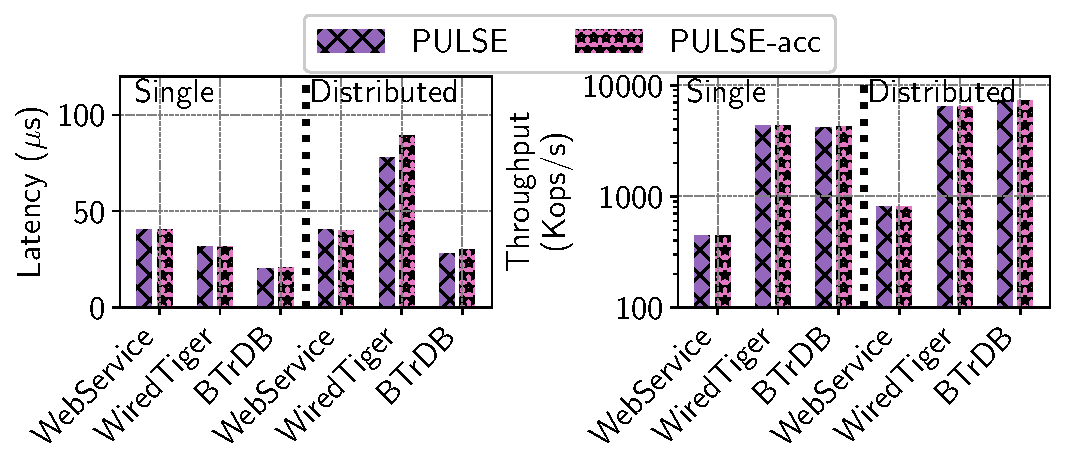
\includegraphics[width=0.4\textwidth]{fig/pulse/breakdown.pdf}%
\vspace{-1em}
\caption{\textbf{Impact of distributed pointer traversals (\S\ref{ssec:breakdown}).}}
\label{fig:eval_breakdown}
\end{figure}

\begin{figure}[t]
  \centering	
  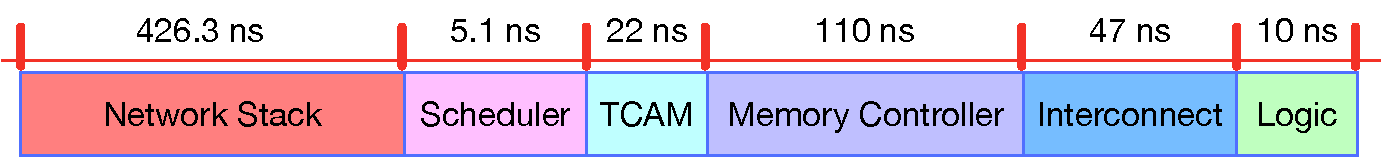
\includegraphics[width=0.48\textwidth]{fig/pulse/breakdown_latency_new.pdf}
  \vspace{-1em}
  \caption{\textbf{Latency breakdown for \name accelerator (\S\ref{ssec:breakdown}).}}
  \label{fig:eval_breakdown_latency_}%\vspace{-1.5em}
\end{figure}




\subsection{Understanding \name Performance}
\label{ssec:breakdown}




\paragraphb{Distributed pointer traversals} We evaluate the impact of distributed pointer traversals (\S\ref{sec:distributed}) by comparing \name against \nameacc, a \name variant that sends requests back to the CPU node if the next pointer is not found on the memory node. Fig.~\ref{fig:eval_breakdown} shows that while both have identical performance on a single memory node, \nameacc observes $1.02$--$1.15\times$ higher latency for two nodes. On the other hand, their throughput is the same since, under sufficient load, memory node bandwidth bottlenecks the system for both.





\paragraphb{Latency breakdown for \name accelerator} 
Fig.~\ref{fig:eval_breakdown_latency_} shows the latency contributions of various hardware components at the \name accelerator for the WebService application. The network stack first processes the pointer traversal request in about $430$ ns, after which the WebService payload is processed by the scheduler and dispatched to an idle memory access pipeline in $5.1$ ns. Then, the memory pipeline takes $\sim$$132$ ns to perform address translation, memory protection, and data fetch from DRAM. Finally, the logic pipeline takes $10$ ns to check the termination conditions and determine the next pointer to look up. This process repeats until the termination condition is met. The time to send a response back over the network stack is symmetric to the request path.












\begin{figure}[t]
\centering
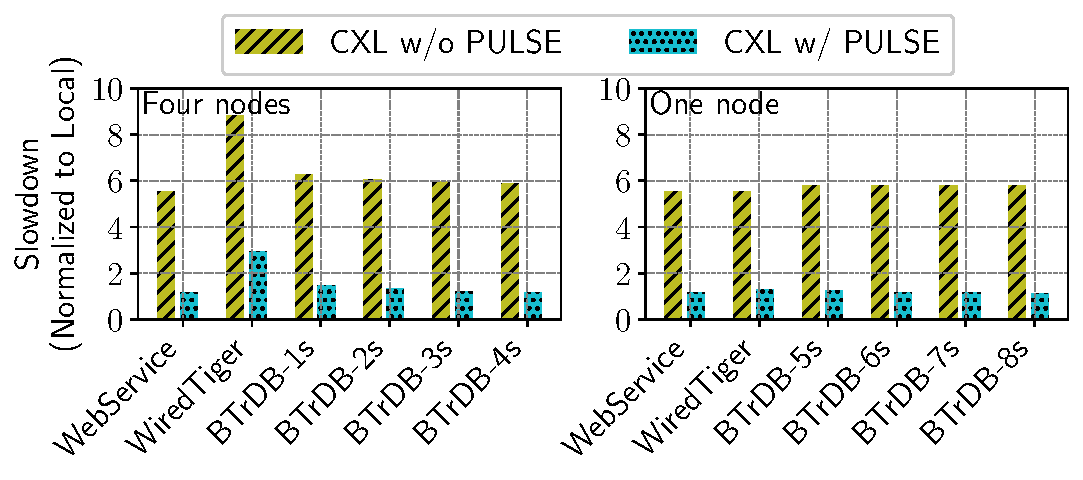
\includegraphics[width=0.9\columnwidth]{fig/pulse/cxl.pdf}
\vspace{-1em}
\caption{
\textbf{Slowdown with simulated CXL interconnect (\S\ref{sec:future}).} 
}

\label{fig:eval_cxl}
\end{figure}

\section{Future Trends and Research}
\label{sec:future}


While \name is implemented atop Ethernet, its design is interconnect-agnostic and could be realized in ASIC-based or FPGA-attached memory devices over emerging interconnects like CXL~\cite{cxl, cxl_azure, sun2023demystifying}. We have verified these benefits in simulation atop detailed memory access and processing traces of our evaluated applications and workloads. The simulator maintains $2$GB of cache in local (CPU-attached) DRAM, while the entire working set is stored on remote CXL memory. Following prior work~\cite{pond}, we model $10$--$20$ns L3 cache latency, $80$ns local DRAM latency, $300$ns CXL-attached memory latency, and $256$B access granularity. We simulate both a four-memory-node setup, which uses a CXL switch with \name logic and a \name accelerator at each memory node, and a single-node setup with no switch. We assume a conservative overhead for \name, using our hardware programmable Ethernet switch and FPGA accelerator latencies.
 
 
Fig.~\ref{fig:eval_cxl} shows the average slowdown for executing our evaluated workloads on CXL memory relative to running it completely locally (\ie, the entire application working set fits in local DRAM) --- with and without \name. In the four-node setup, \name reduces CXL's slowdown by $19$--$33$\% across all applications. 

In the single-node setup, \name still reduces the slowdown by $19$--$23$\% by minimizing high-latency traversals over the CXL interconnect. While a real hardware realization is necessary to precisely quantify \name's benefits, our simulation (which models the lowest possible CXL latency and highest possible \name overheads) highlights its potential for improving performance in emerging interconnects.

